\newpage

\section{Реализация системы}

\subsection{Докеризация}

Чтобы использовать MySQL нам нужно устанавливать LAMP (Linux, Apache, MySQL, PHP).
Это будет не удобно, если нужно будет разварачивать на нескольких компьютерах,
так как ручной ввод команд будет занимать много времени.
Чтобы автоматизировать ввод команд в курсовом проекте использовался Docker и docker-compose.

Вместо Docker и docker-compose можно было использовать решения, такие как Denwer и OpenServer,
но для этого нам нужно иметь эти программы на каждом компьютере. Имея один файл docker-compose
в проекте убивает проблему установки больших дистрибутивов, таких как OpenServer.

\subsubsection*{Установка Docker на Windows 10}

\begin{itemize}
    \item[1.] Заходим на Wikipedia и находим оффициальный сайт Docker. \\
    \url{https://ru.wikipedia.org/wiki/Docker} \\
    Находим ссылку <<Сайт docker.com>> - и переходим по ней. \\
    Скриншот на \textbf{рис.~\ref{fig:gpi_pz_docker_01} (стр. \pageref{fig:gpi_pz_docker_01})}.

    \item[2.] Открываем оффициальный сайт Docker. \\
    \url{https://www.docker.com/} \\
    Переходим на страницу загрузки, нажав на кнопку <<Get Started>>. \\
    \url{https://www.docker.com/get-started} \\
    Скриншот на \textbf{рис.~\ref{fig:gpi_pz_docker_02} (стр. \pageref{fig:gpi_pz_docker_02})}.

    \item[3.] Выбираем установщик для Windows. \\
    Скриншот на \textbf{рис.~\ref{fig:gpi_pz_docker_03} (стр. \pageref{fig:gpi_pz_docker_03})}.

    \item[4.] Запускаем установщик Windows. \\
    Скриншот на \textbf{рис.~\ref{fig:gpi_pz_docker_04} (стр. \pageref{fig:gpi_pz_docker_04})}.

    \item[5.] После установки Docker, установщик просит перезагрузить компьютер.
    Перезагружаем компьютер нажав на кнопку <<Close and restart>>. \\
    Скриншот на \textbf{рис.~\ref{fig:gpi_pz_docker_05} (стр. \pageref{fig:gpi_pz_docker_05})}.

    \item[6.] После перезагрузки компюьтера Docker автоматически запустился и просит принять лицензию.
    Соглашаемся с лицензией поставив галочку.
    Продолжаем запуск нажав на кнопку <<Accept>>.
    Скриншот на \textbf{рис.~\ref{fig:gpi_pz_docker_06} (стр. \pageref{fig:gpi_pz_docker_06})}.

    \item[7.] При запуске Docker возникает ошибка.
    Эта ошибка возникает из-за того, что у нас установлен WSL версии 1. \\
    Ошибка просит посетить сайт: \url{https://aka.ms/wsl2kernel}. \\
    Скриншот на \textbf{рис.~\ref{fig:gpi_pz_docker_07} (стр. \pageref{fig:gpi_pz_docker_07})}.

    \item[8.] По переходу по ссылке \url{https://aka.ms/wsl2kernel} происходит перенаправление
    на страницу с инструкцией об установке обновления WSL2.
    На это странице находим ссылку на загрузку установщика. \\
    Скриншот на \textbf{рис.~\ref{fig:gpi_pz_docker_08} (стр. \pageref{fig:gpi_pz_docker_08})}.

    \item[9.] Запускаем установщик. Жмём кнопку <<Next>>. \\
    Скриншот на \textbf{рис.~\ref{fig:gpi_pz_docker_09} (стр. \pageref{fig:gpi_pz_docker_09})}.
    
    \item[10.] Завершаем установку. Жмём кнопку <<Finish>>. \\
    Скриншот на \textbf{рис.~\ref{fig:gpi_pz_docker_10} (стр. \pageref{fig:gpi_pz_docker_10})}.

    \item[11.] Возврашаемся к инструкции на сайте. Эта инструкция говорит нам поменять WSL1 на WSL2,
    прописав команду в Power Shell. Копируем команду нажав на кнопку <<Copy>>. \\
    Скриншот на \textbf{рис.~\ref{fig:gpi_pz_docker_11} (стр. \pageref{fig:gpi_pz_docker_11})}.

    \item[12.] Чтобы открыть Power Shell ищем его в поиске.
    Чтобы открыть поиск зажимает клавиши <<Win>> + <<Q>>.
    В поиске прописываем <<powershell>>. Запускаем Power Shell нажав кнопку <<Open>>. \\
    Скриншот на \textbf{рис.~\ref{fig:gpi_pz_docker_12} (стр. \pageref{fig:gpi_pz_docker_12})}.

    \item[13.] Открывается Power Shell. Вставляем команду. \\
    Скриншот на \textbf{рис.~\ref{fig:gpi_pz_docker_13} (стр. \pageref{fig:gpi_pz_docker_13})}.

    \item[14.] Перезагружаем компьютер - и теперь Docker запускается без ошибки.
    Но для того, чтобы мы могли воспользоваться командами <<docker>> и <<docker-compose>>
    нам нужен какой-нибудь дистрибутив Linux. \\
    Скриншот на \textbf{рис.~\ref{fig:gpi_pz_docker_14} (стр. \pageref{fig:gpi_pz_docker_14})}.

    \item[15.] Если вернуться к инструкции, то инструкция также рекомендует нам установть
    какой-нибудь дистрибутив Linux. \\
    Скриншот на \textbf{рис.~\ref{fig:gpi_pz_docker_15} (стр. \pageref{fig:gpi_pz_docker_15})}.

    \item[16.] Нам нужен магазин приложений. Найдем его через поиск.
    Чтобы открыть поиск зажимает клавиши <<Win>> + <<Q>>.
    В поиске пишем <<Store>>.
    Открываем, нажав клавишу <<Open>>. \\
    Скриншот на \textbf{рис.~\ref{fig:gpi_pz_docker_16} (стр. \pageref{fig:gpi_pz_docker_16})}.

    \item[17.] В магизине приложении в поиске вводим <<Ubuntu>>.
    Переходим на стриницу приложения Ubuntu нажав на нужный вариант из предложенных. \\
    Скриншот на \textbf{рис.~\ref{fig:gpi_pz_docker_17} (стр. \pageref{fig:gpi_pz_docker_17})}.

    \item[18.] На странице загрузки жмём кнопку <<Get>> для того, чтобы установить приложение на компьютер. \\
    Скриншот на \textbf{рис.~\ref{fig:gpi_pz_docker_18} (стр. \pageref{fig:gpi_pz_docker_18})}.

    \item[19.] Открываем терминал Ubuntu, например, через поиск. Жмём <<Win>> + <<R>>.
    В поиске вводим <<Ubuntu>>. Жмём <<Open>>.
    При первом запуске терминала Ubuntu дистрибутив будет устанавлився.
    При установке просят придумать имя пользователя на английском. Вводим имя пользователя.
    Просят ввести пароль.
    Когда мы будет вводим вводить пароль, то символы не будут отображаться - это сделано в целях безопасности.
    Далее системы будет готова к использованию. \\ 
    Скриншот на \textbf{рис.~\ref{fig:gpi_pz_docker_19} (стр. \pageref{fig:gpi_pz_docker_19})}.
    
    \item[20.] Как уже скачали выбранный дистрибутив (в нашем случае Ubuntu),
    то в приложении <<Docker Desktop>> нужно включить наш дистрибутив.
    \begin{itemize}
        \item[1.] Запускаем <<Docker Desktop>>.
        \item[2.] Переходим в настройки нажав на шестиренку.
        \item[3.] Переходим в раздел <<Resources>>.
        \item[4.] Переходим в подпункт <<WSL INTEGRATION>>.
        \item[5.] Ставим ползунок к <<Ubuntu>>.
    \end{itemize}
    Скриншот на \textbf{рис.~\ref{fig:gpi_pz_docker_20} (стр. \pageref{fig:gpi_pz_docker_20})}.

    \item[21.] Запускаем терминал Ubuntu через поиск. Открываем поиск нажав <<Win>> + <<R>>. \\
    В поиске вводим <<Ubuntu>>. Жмём кнопку <<Open>>. \\
    Скриншот на \textbf{рис.~\ref{fig:gpi_pz_docker_21} (стр. \pageref{fig:gpi_pz_docker_21})}.

    \item[22.] В терминале Ubuntu вводим команду <<docker -v>> - и у нас выводится его версия <<Docker version 20.10.11, build dea9396>>,
    то есть у нас установлен Docker. \\
    В терминале Ubuntu вводим команду <<docker-compose -v>> - и у нас выводится его версия <<Docker Compose version v2.2.1>>,
    то есть у нас установлен docker-compose. \\
    Скриншот на \textbf{рис.~\ref{fig:gpi_pz_docker_22} (стр. \pageref{fig:gpi_pz_docker_22})}.

\end{itemize}

\begin{figure}[!p]
    \centering
    \begin{minipage}{0.47\textwidth}
        \centering
        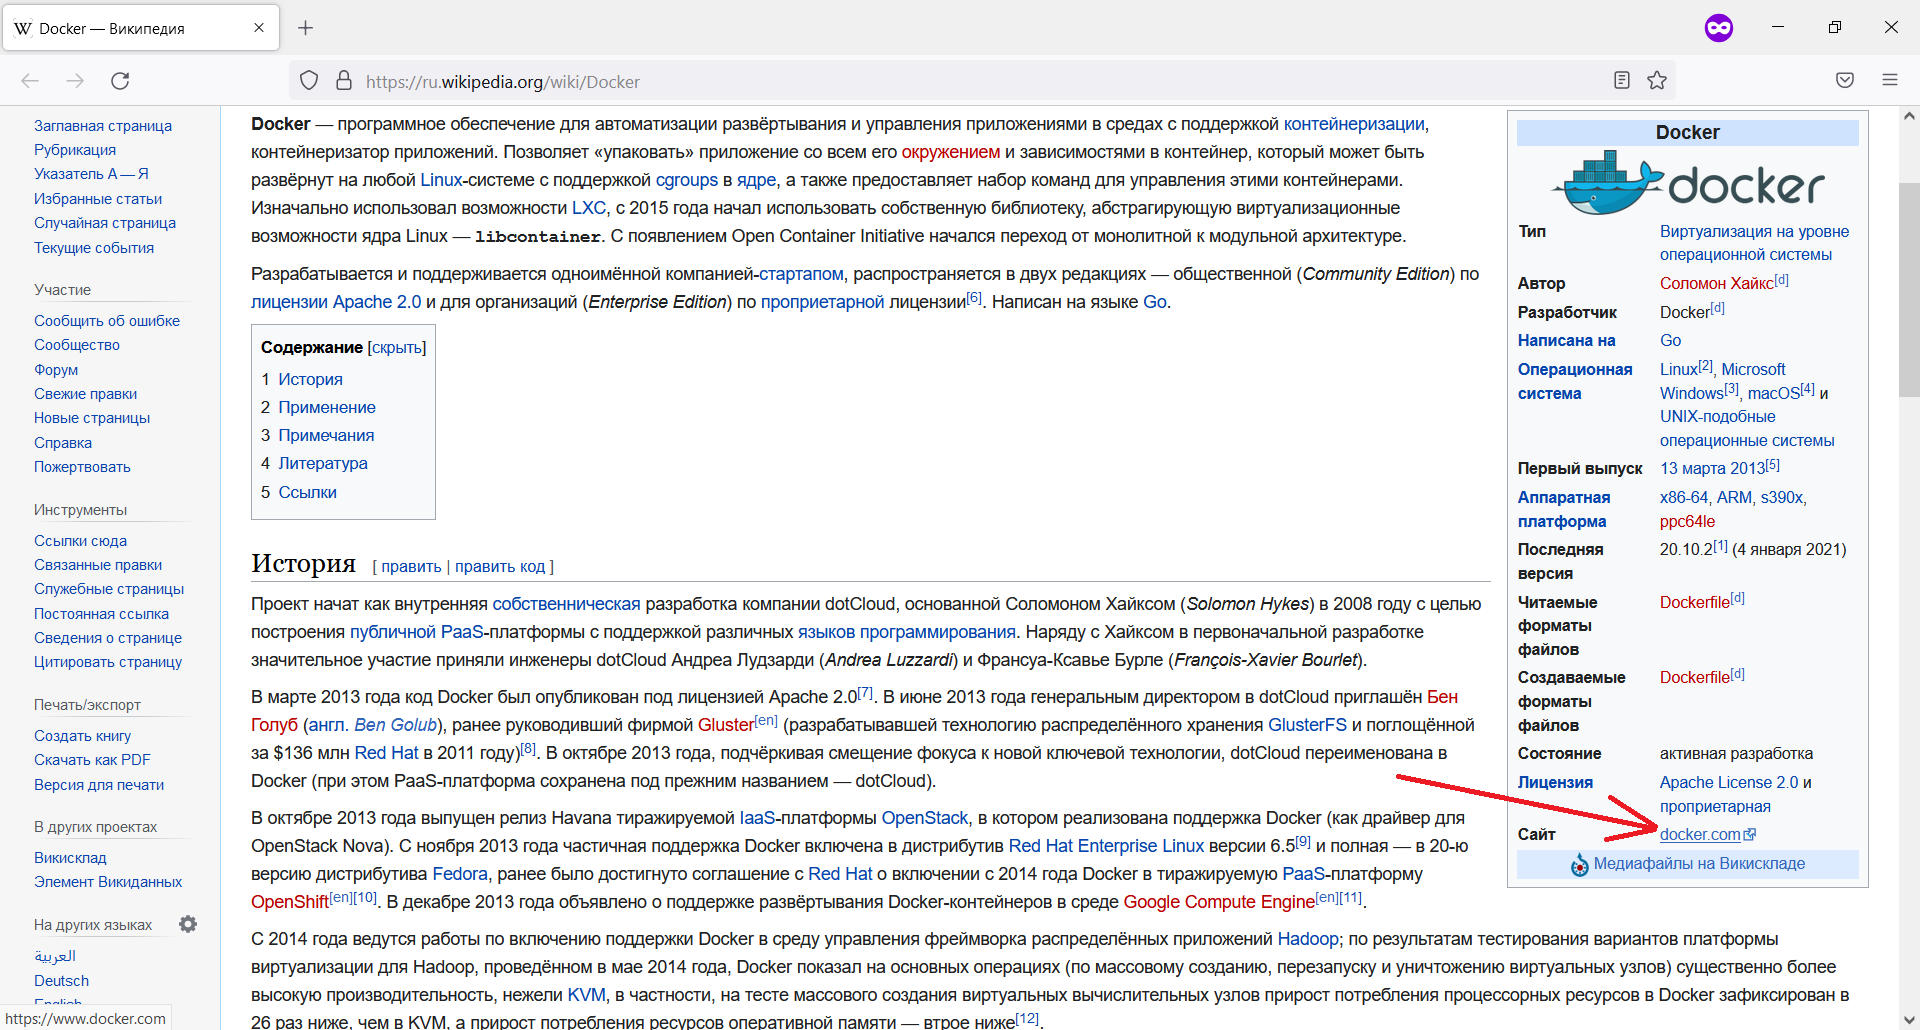
\includegraphics[width=\linewidth]
            {_assets/gpi_pz_docker_01.png}
        \caption{Находим сайт на Wikipedia}
        \label{fig:gpi_pz_docker_01}
    \end{minipage}
    \begin{minipage}{0.47\textwidth}
        \centering
        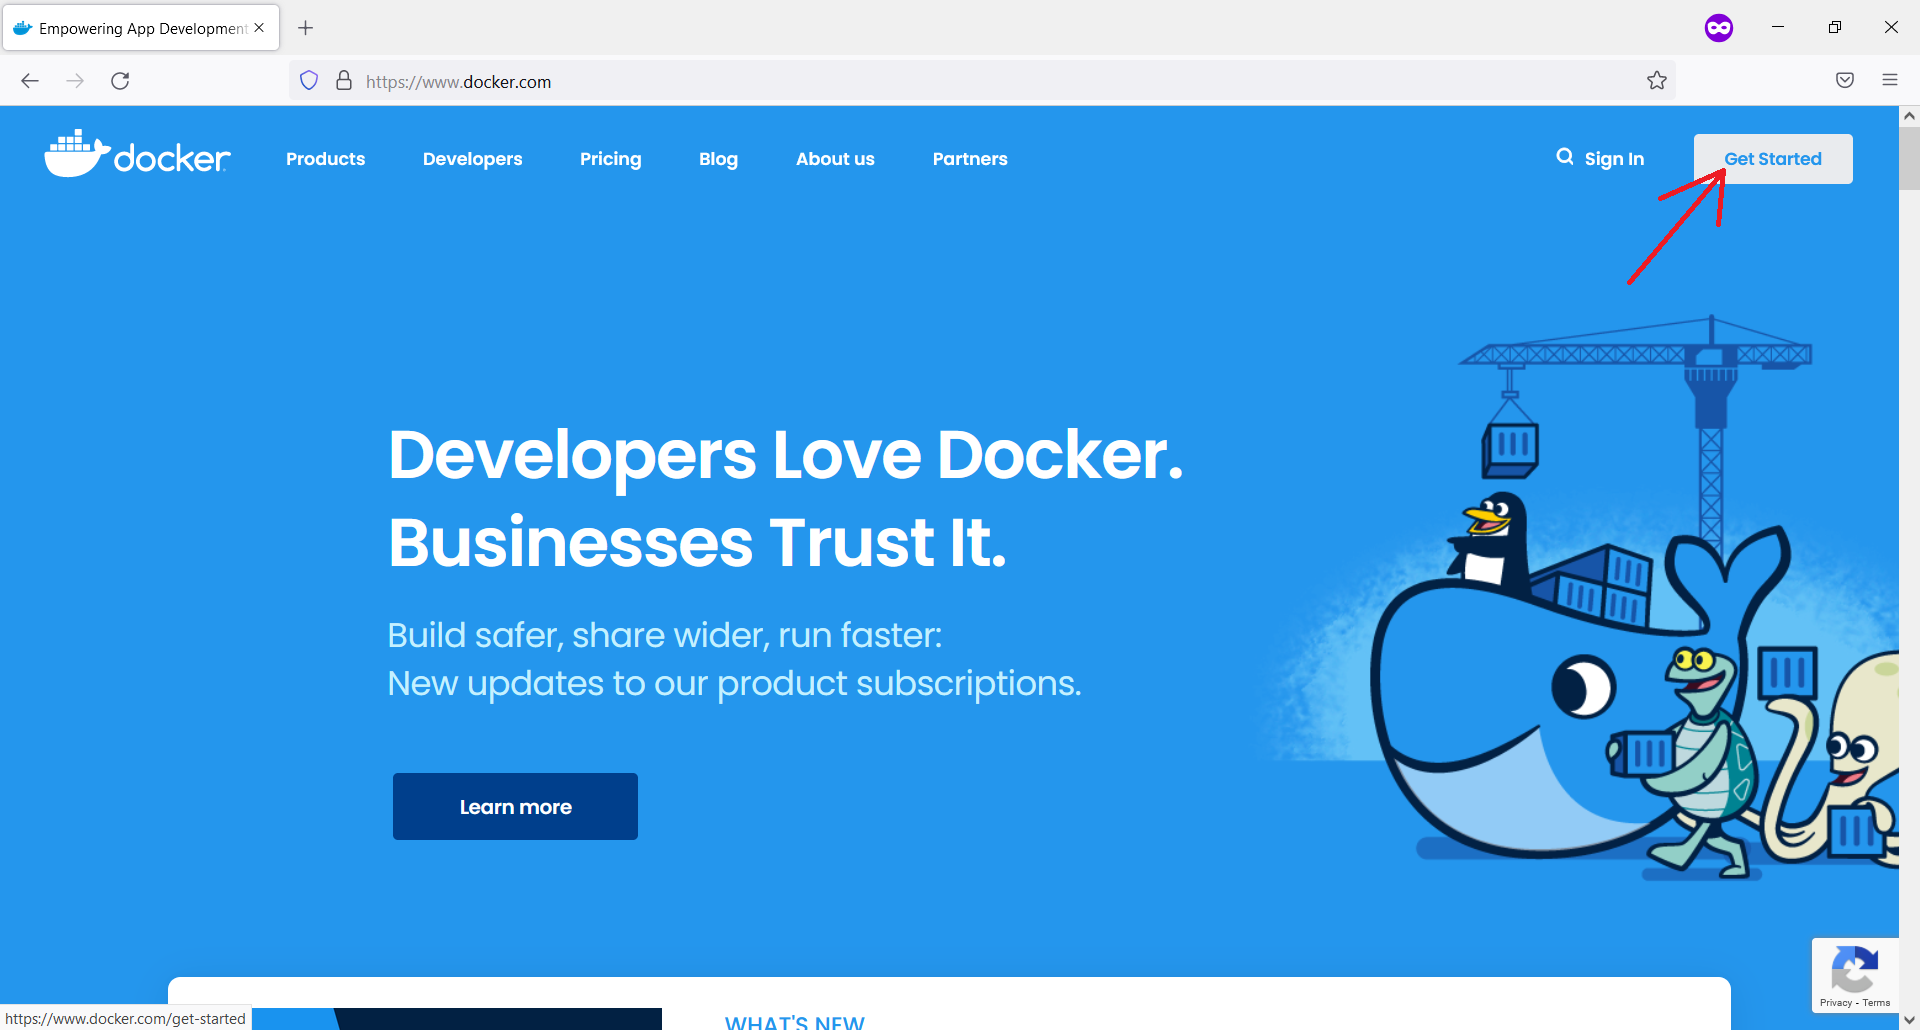
\includegraphics[width=\linewidth]
            {_assets/gpi_pz_docker_02.png}
        \caption{Открываем сайт}
        \label{fig:gpi_pz_docker_02}
    \end{minipage}
\end{figure}

\begin{figure}[!p]
    \centering
    \begin{minipage}{0.47\textwidth}
        \centering
        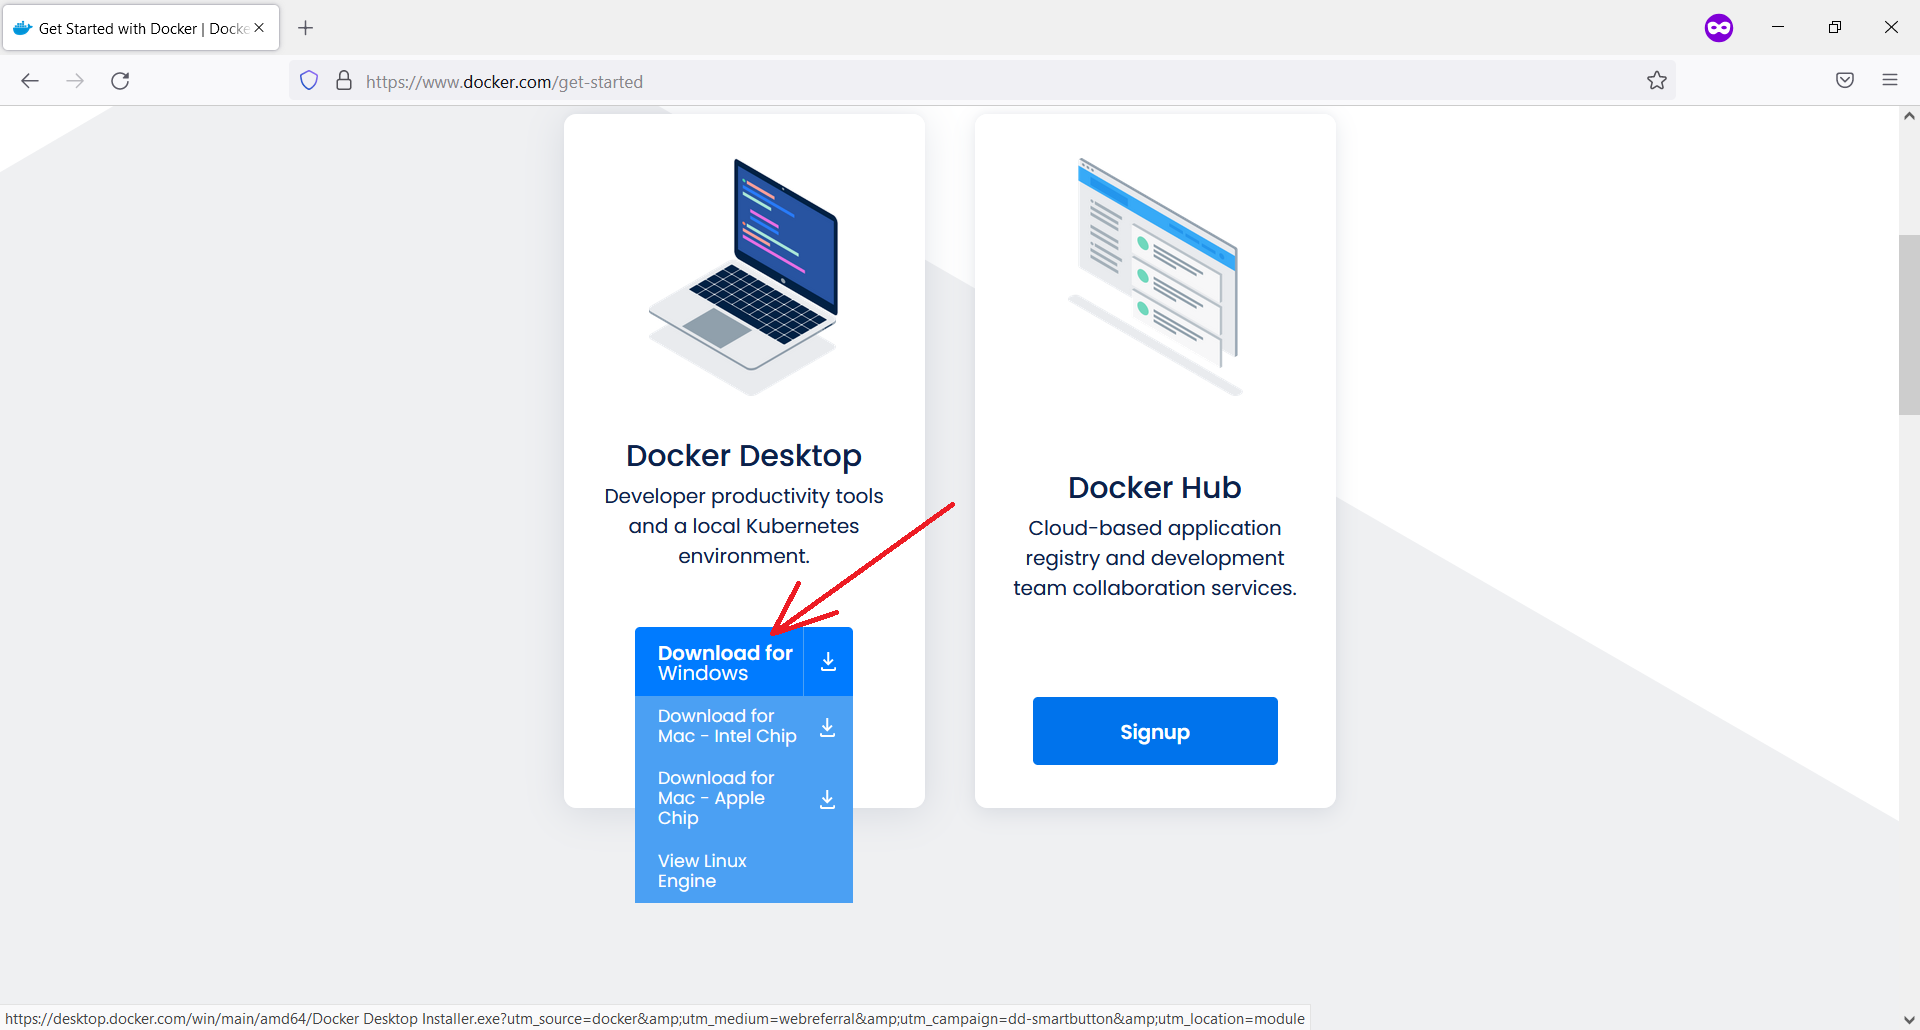
\includegraphics[width=\linewidth]
            {_assets/gpi_pz_docker_03.png}
        \caption{Выбираем установщик Windows}
        \label{fig:gpi_pz_docker_03}
    \end{minipage}
    \begin{minipage}{0.47\textwidth}
        \centering
        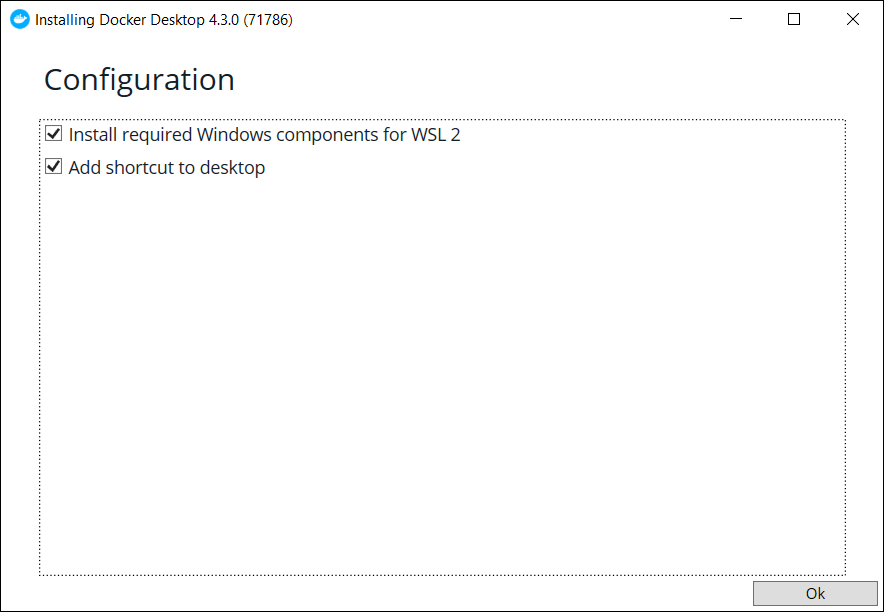
\includegraphics[width=\linewidth]
            {_assets/gpi_pz_docker_04.png}
        \caption{Запускаем файл и устанавливаем Docker}
        \label{fig:gpi_pz_docker_04}
    \end{minipage}
\end{figure}

\begin{figure}[!p]
    \centering
    \begin{minipage}{0.47\textwidth}
        \centering
        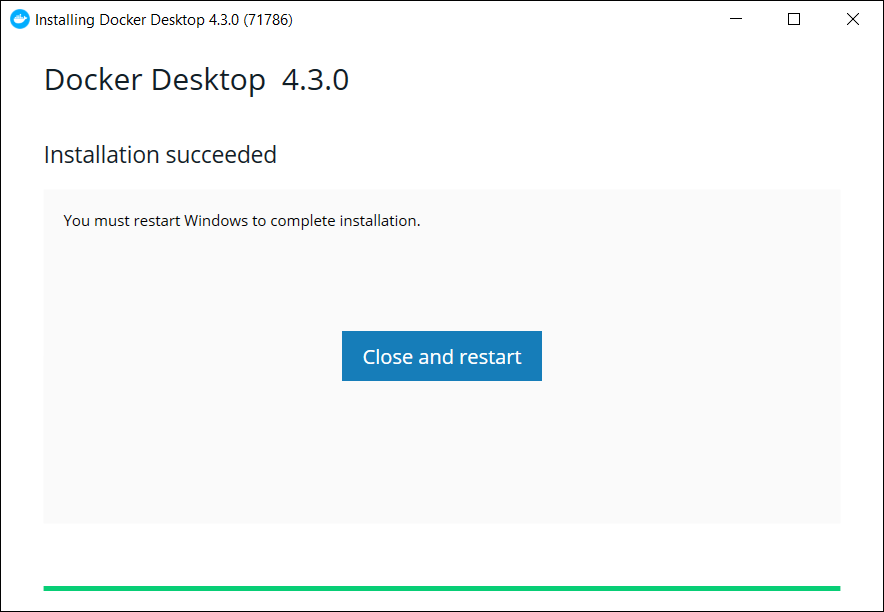
\includegraphics[width=\linewidth]
            {_assets/gpi_pz_docker_05.png}
        \caption{Перезагружаем компьютер}
        \label{fig:gpi_pz_docker_05}
    \end{minipage}
    \begin{minipage}{0.47\textwidth}
        \centering
        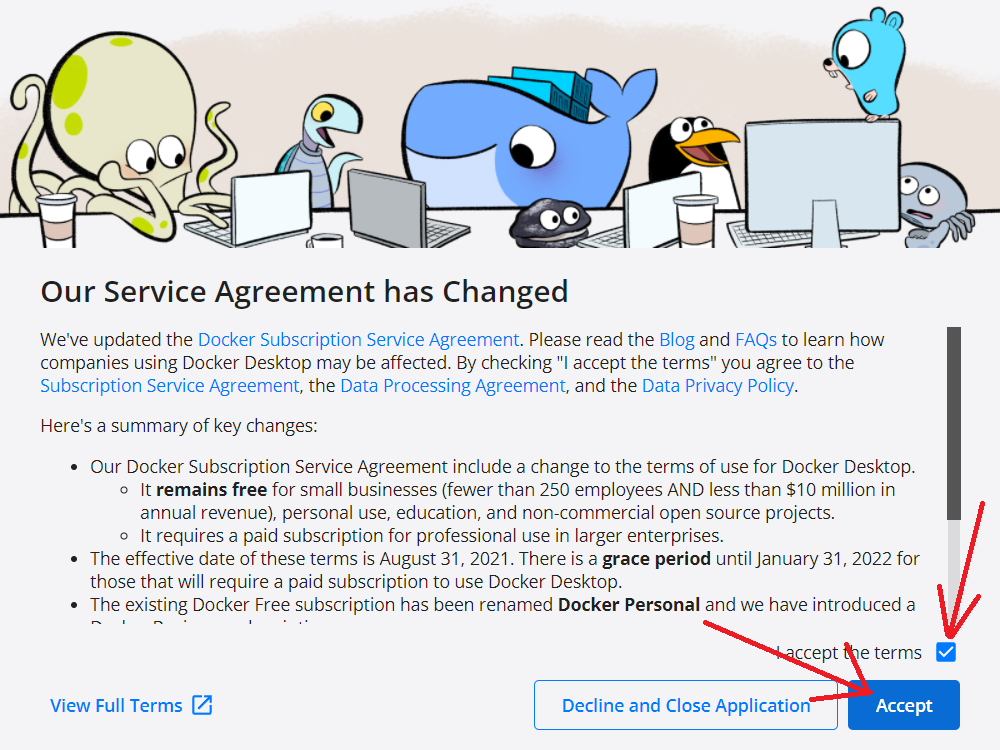
\includegraphics[width=\linewidth]
            {_assets/gpi_pz_docker_06.png}
        \caption{Принимаем лицензию}
        \label{fig:gpi_pz_docker_06}
    \end{minipage}
\end{figure}

\begin{figure}[!p]
    \centering
    \begin{minipage}{0.47\textwidth}
        \centering
        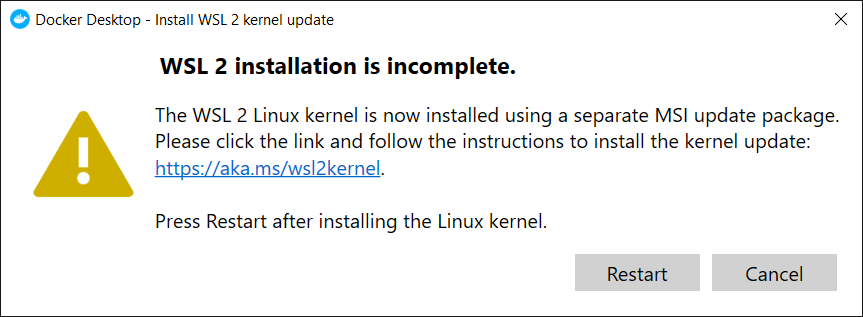
\includegraphics[width=\linewidth]
            {_assets/gpi_pz_docker_07.png}
        \caption{Ошибка (нет WSL2). Переходим на сайт}
        \label{fig:gpi_pz_docker_07}
    \end{minipage}
    \begin{minipage}{0.47\textwidth}
        \centering
        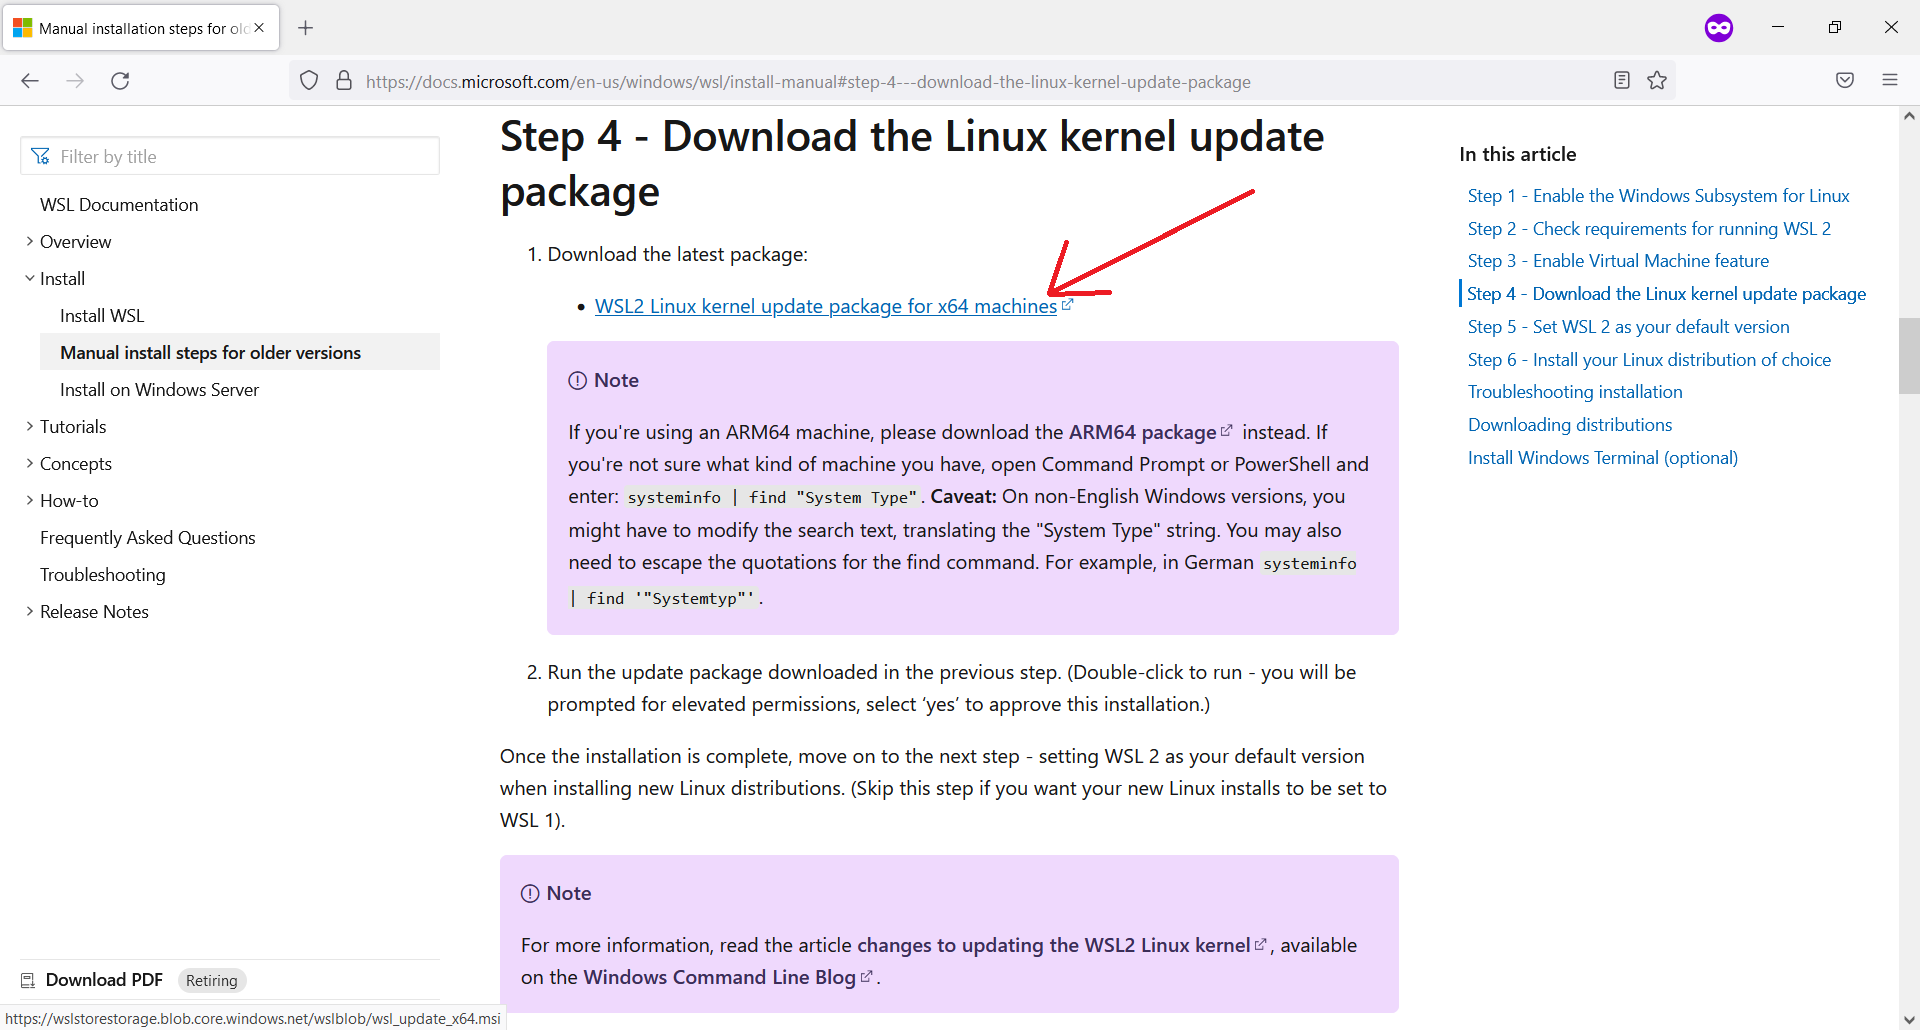
\includegraphics[width=\linewidth]
            {_assets/gpi_pz_docker_08.png}
        \caption{Качаем WSL2 с сайта}
        \label{fig:gpi_pz_docker_08}
    \end{minipage}
\end{figure}

\begin{figure}[!p]
    \centering
    \begin{minipage}{0.47\textwidth}
        \centering
        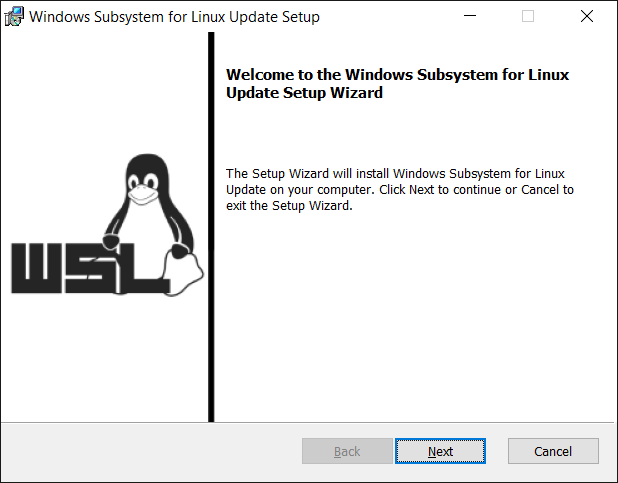
\includegraphics[width=\linewidth]
            {_assets/gpi_pz_docker_09.png}
        \caption{Устанавливаем обновление WSL2}
        \label{fig:gpi_pz_docker_09}
    \end{minipage}
    \begin{minipage}{0.47\textwidth}
        \centering
        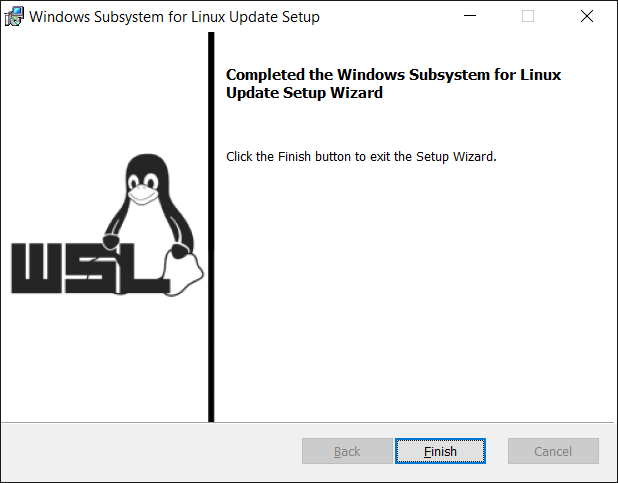
\includegraphics[width=\linewidth]
            {_assets/gpi_pz_docker_10.png}
        \caption{Устанавливаем обновление WSL2}
        \label{fig:gpi_pz_docker_10}
    \end{minipage}
\end{figure}

\begin{figure}[!p]
    \centering
    \begin{minipage}{0.47\textwidth}
        \centering
        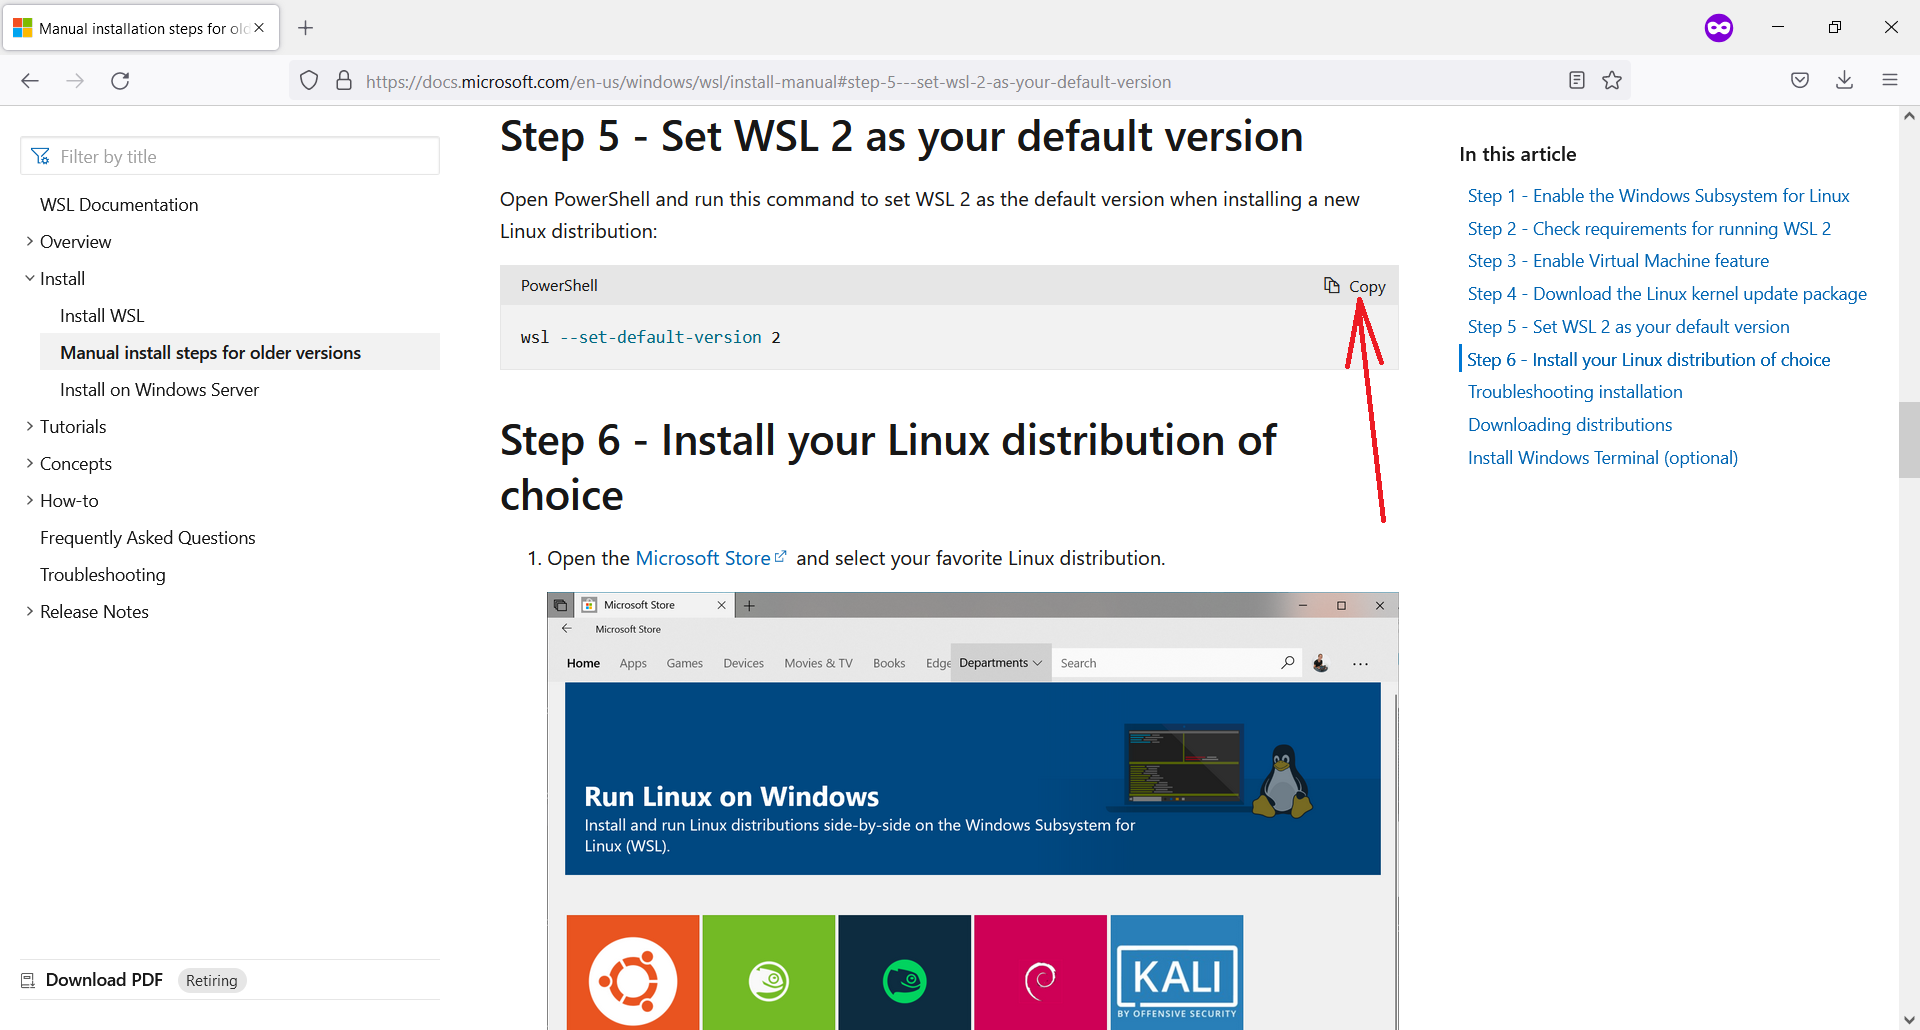
\includegraphics[width=\linewidth]
            {_assets/gpi_pz_docker_11.png}
        \caption{Копируем команду Power Shell, которая поменяет WSL1 на WSL2}
        \label{fig:gpi_pz_docker_11}
    \end{minipage}
    \begin{minipage}{0.47\textwidth}
        \centering
        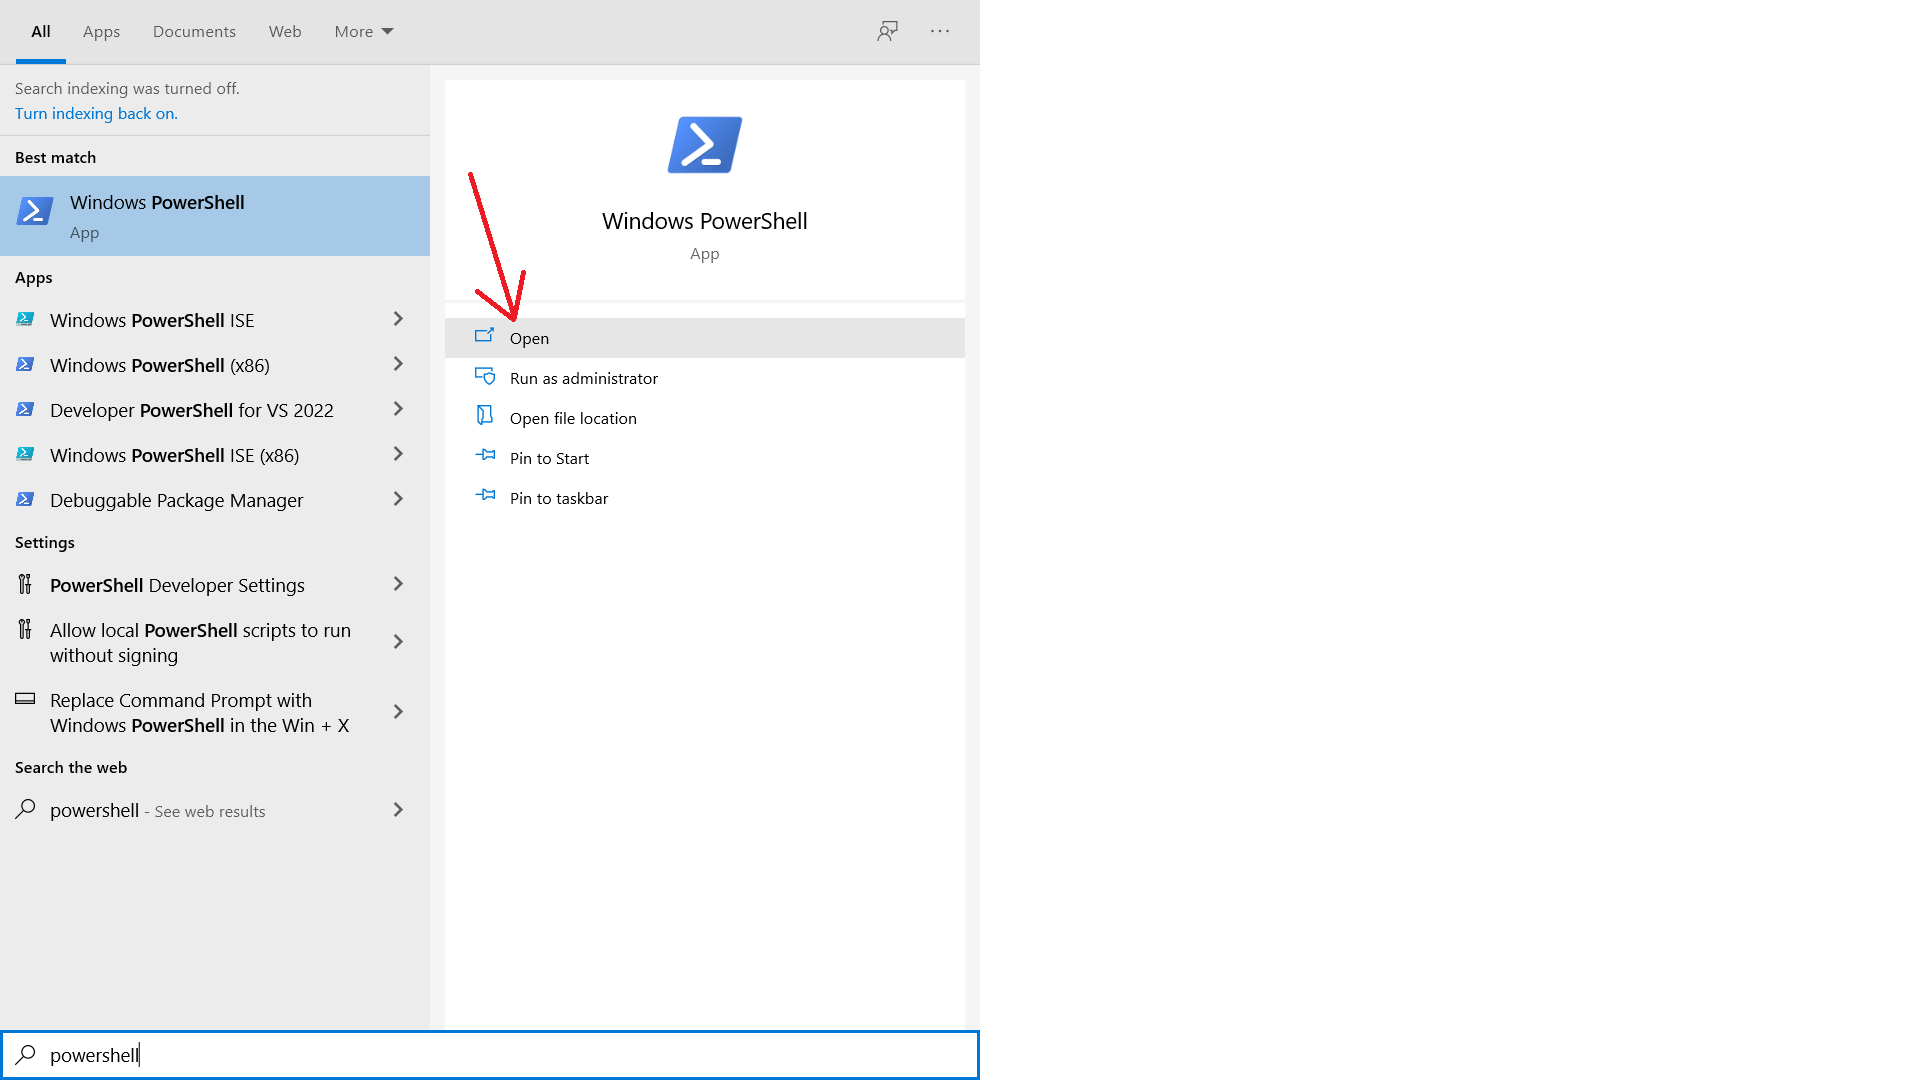
\includegraphics[width=\linewidth]
            {_assets/gpi_pz_docker_12.png}
        \caption{Запускаем поиск, нажав <<Win>> + <<Q>>. Вводим <<powershell>>}
        \label{fig:gpi_pz_docker_12}
    \end{minipage}
\end{figure}

\begin{figure}[!p]
    \centering
    \begin{minipage}{0.47\textwidth}
        \centering
        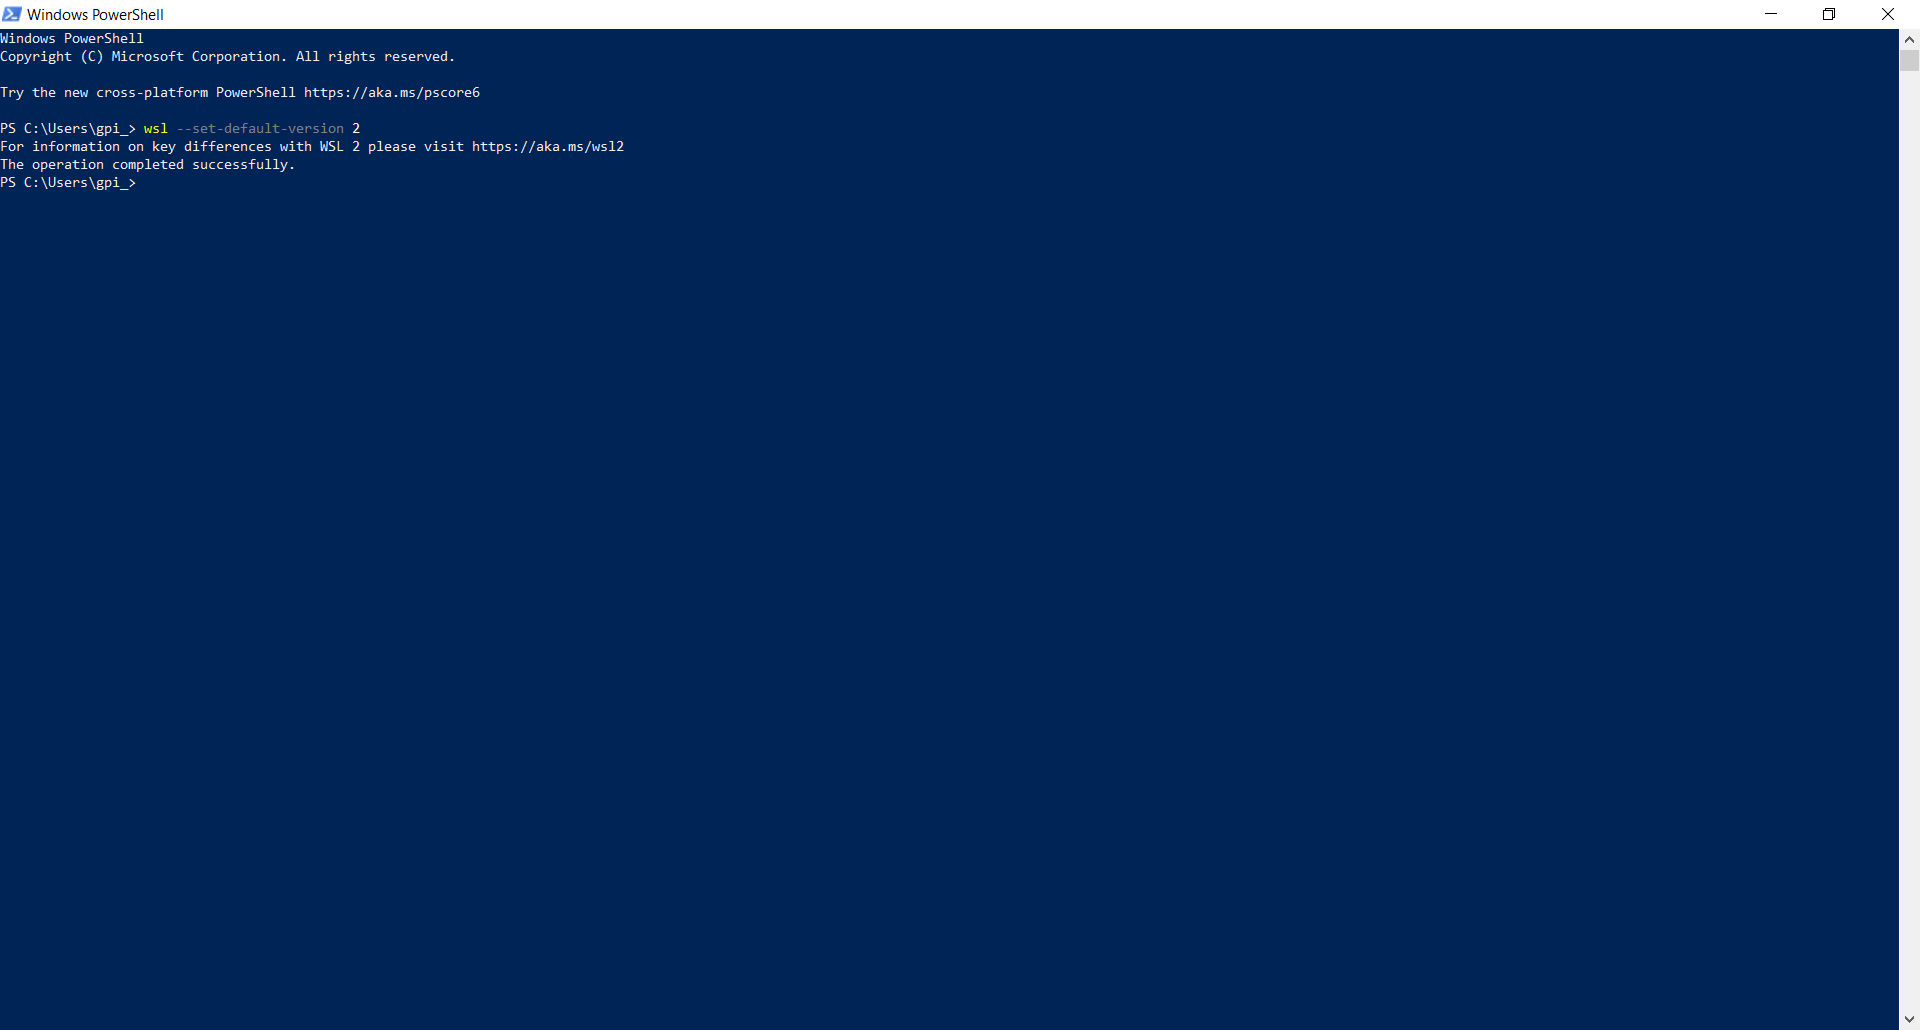
\includegraphics[width=\linewidth]
            {_assets/gpi_pz_docker_13.png}
        \caption{В Power Shell вставляем скопированную команду. \\ Нажимаем <<Enter>> для выполнения}
        \label{fig:gpi_pz_docker_13}
    \end{minipage}
    \begin{minipage}{0.47\textwidth}
        \centering
        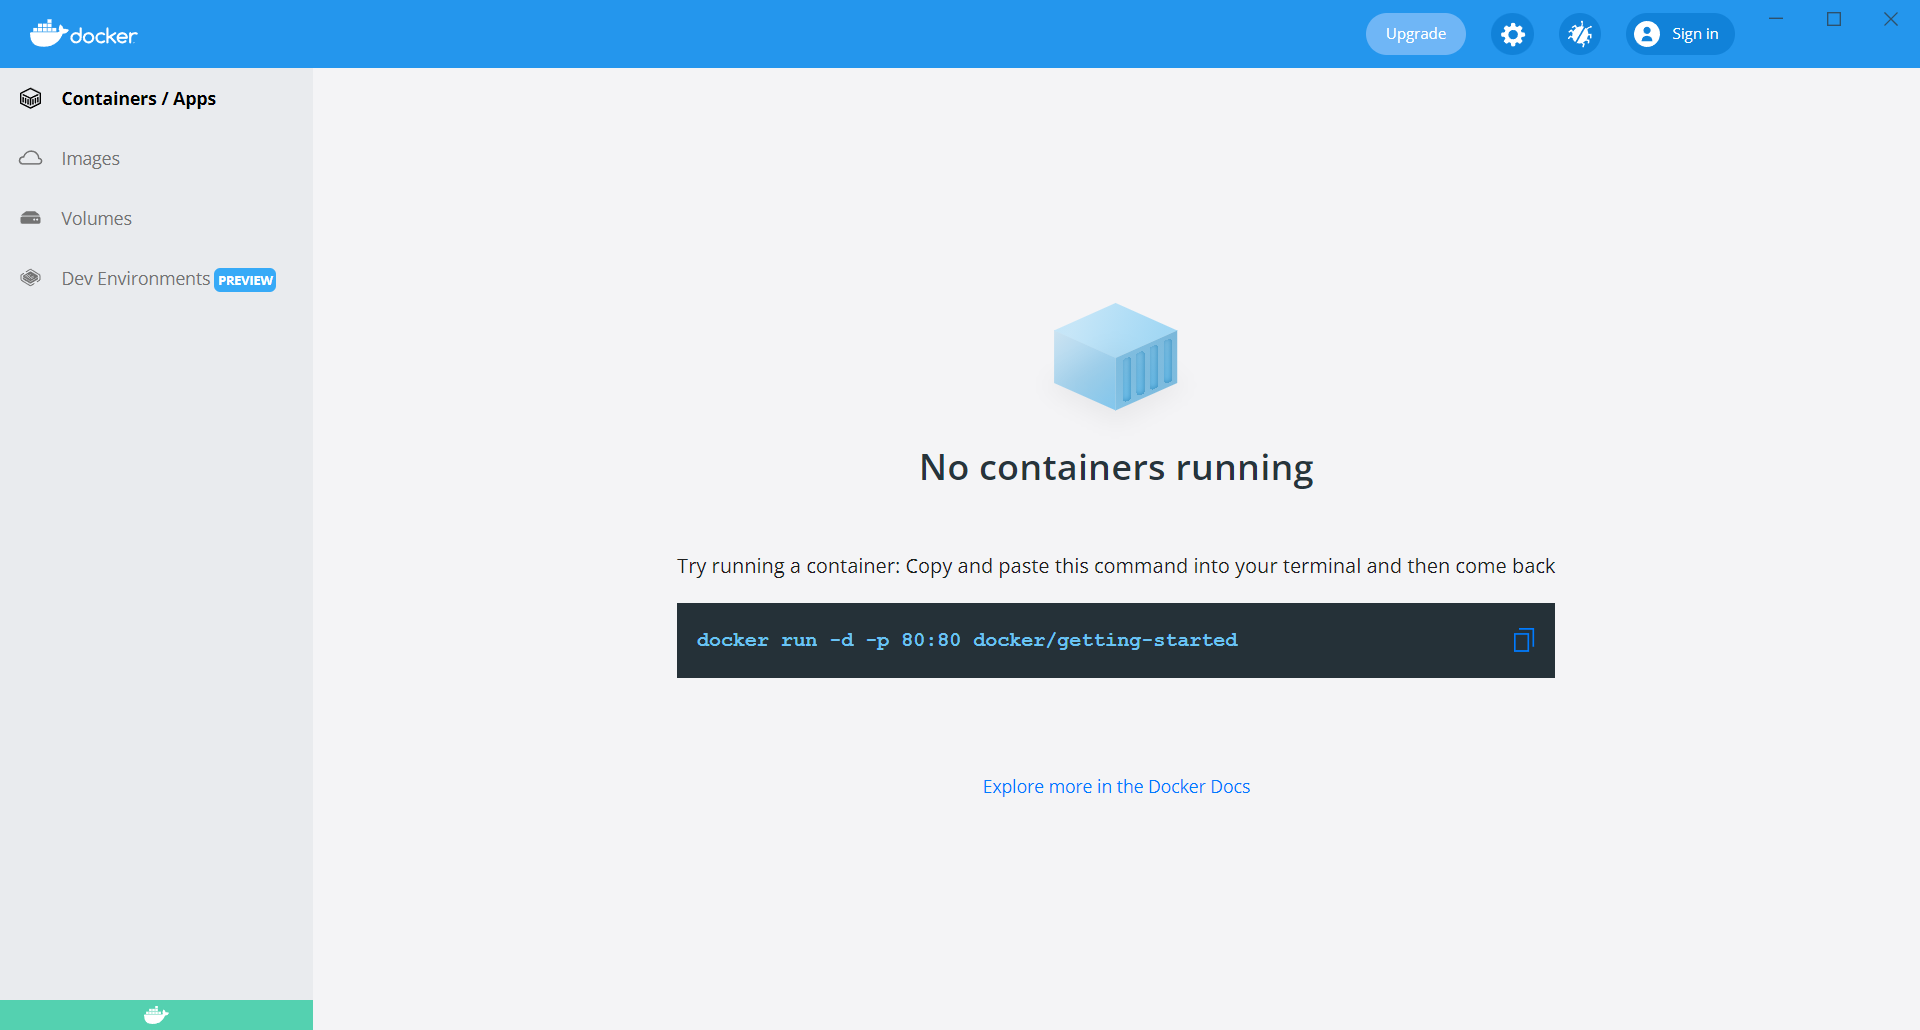
\includegraphics[width=\linewidth]
            {_assets/gpi_pz_docker_14.png}
        \caption{<<Docker Desktop>> запускается без ошибки \\ (но у нас пока нет дистрибутива)}
        \label{fig:gpi_pz_docker_14}
    \end{minipage}
\end{figure}

\begin{figure}[!p]
    \centering
    \begin{minipage}{0.47\textwidth}
        \centering
        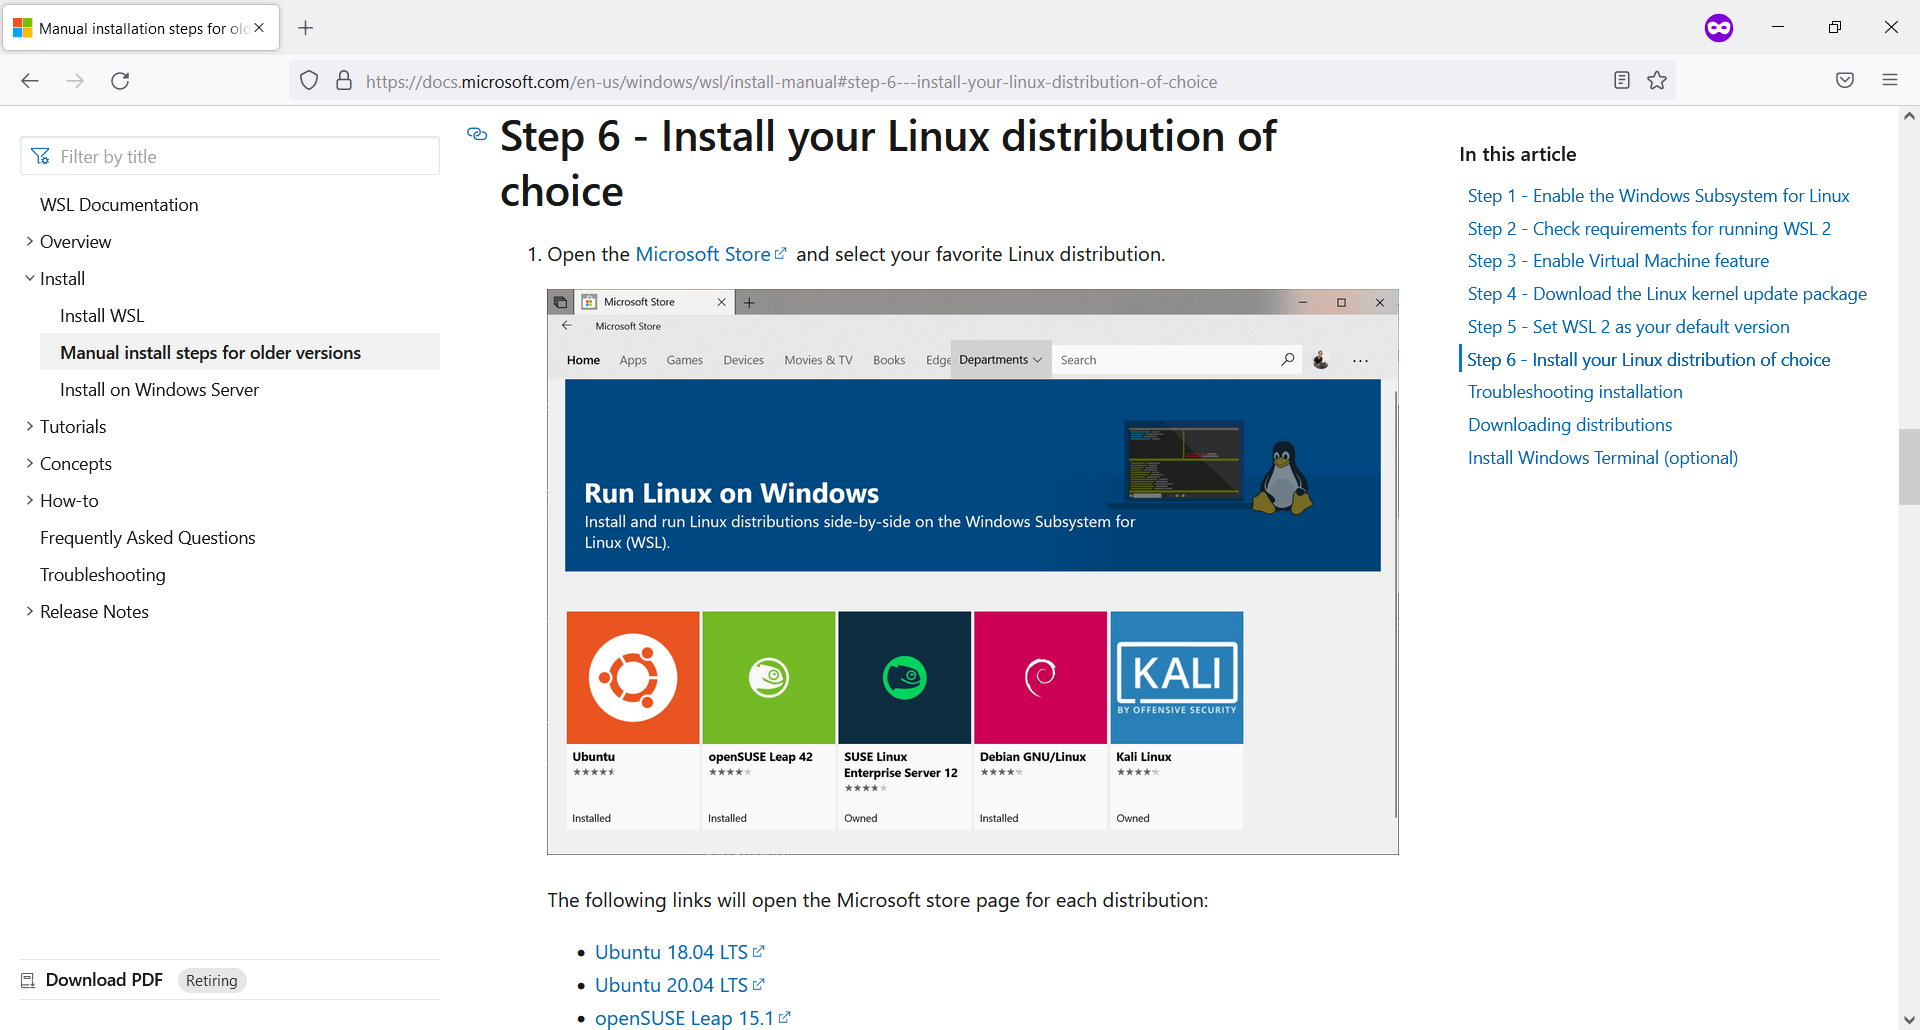
\includegraphics[width=\linewidth]
            {_assets/gpi_pz_docker_15.png}
        \caption{Инструкция говорит скачать дистрибутив Linux}
        \label{fig:gpi_pz_docker_15}
    \end{minipage}
    \begin{minipage}{0.47\textwidth}
        \centering
        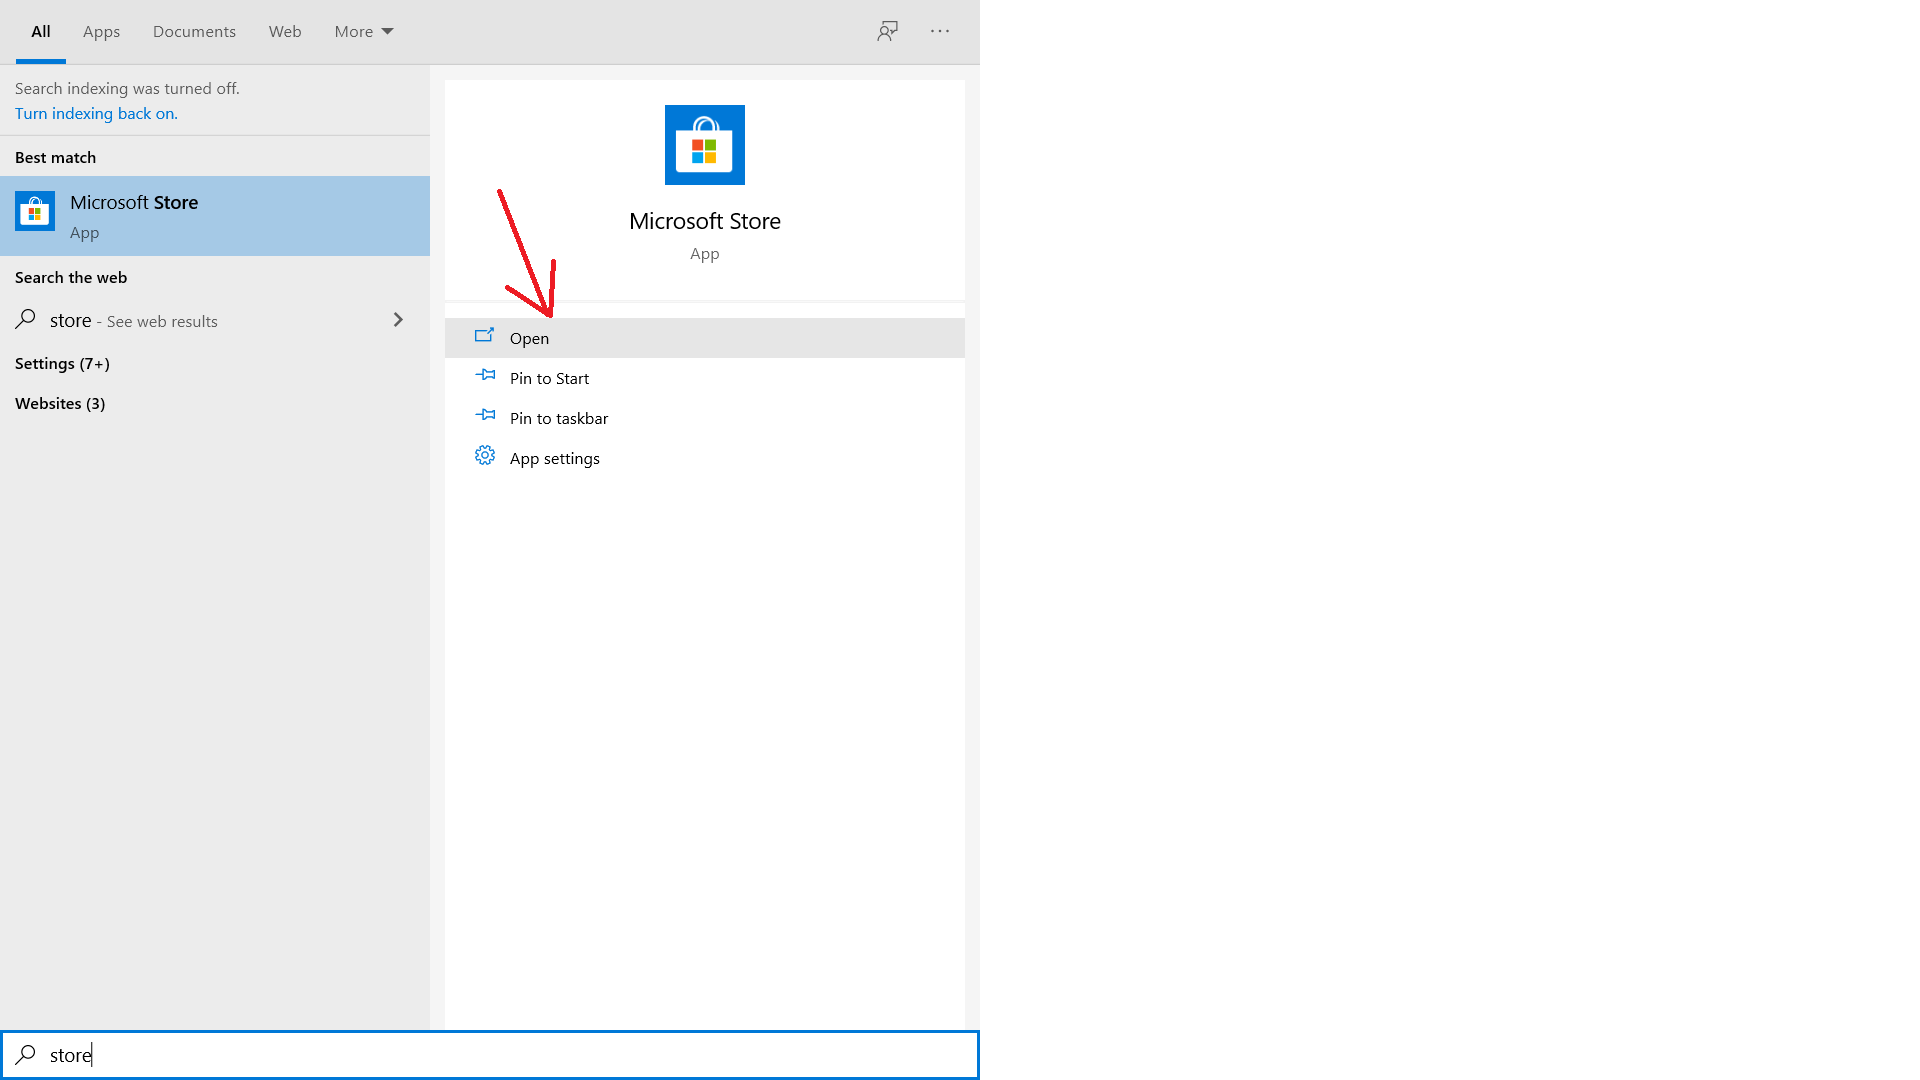
\includegraphics[width=\linewidth]
            {_assets/gpi_pz_docker_16.png}
        \caption{Запускаем поиск, нажав Win + Q, - и вводим <<Store>>}
        \label{fig:gpi_pz_docker_16}
    \end{minipage}
\end{figure}

\begin{figure}[!p]
    \centering
    \begin{minipage}{0.47\textwidth}
        \centering
        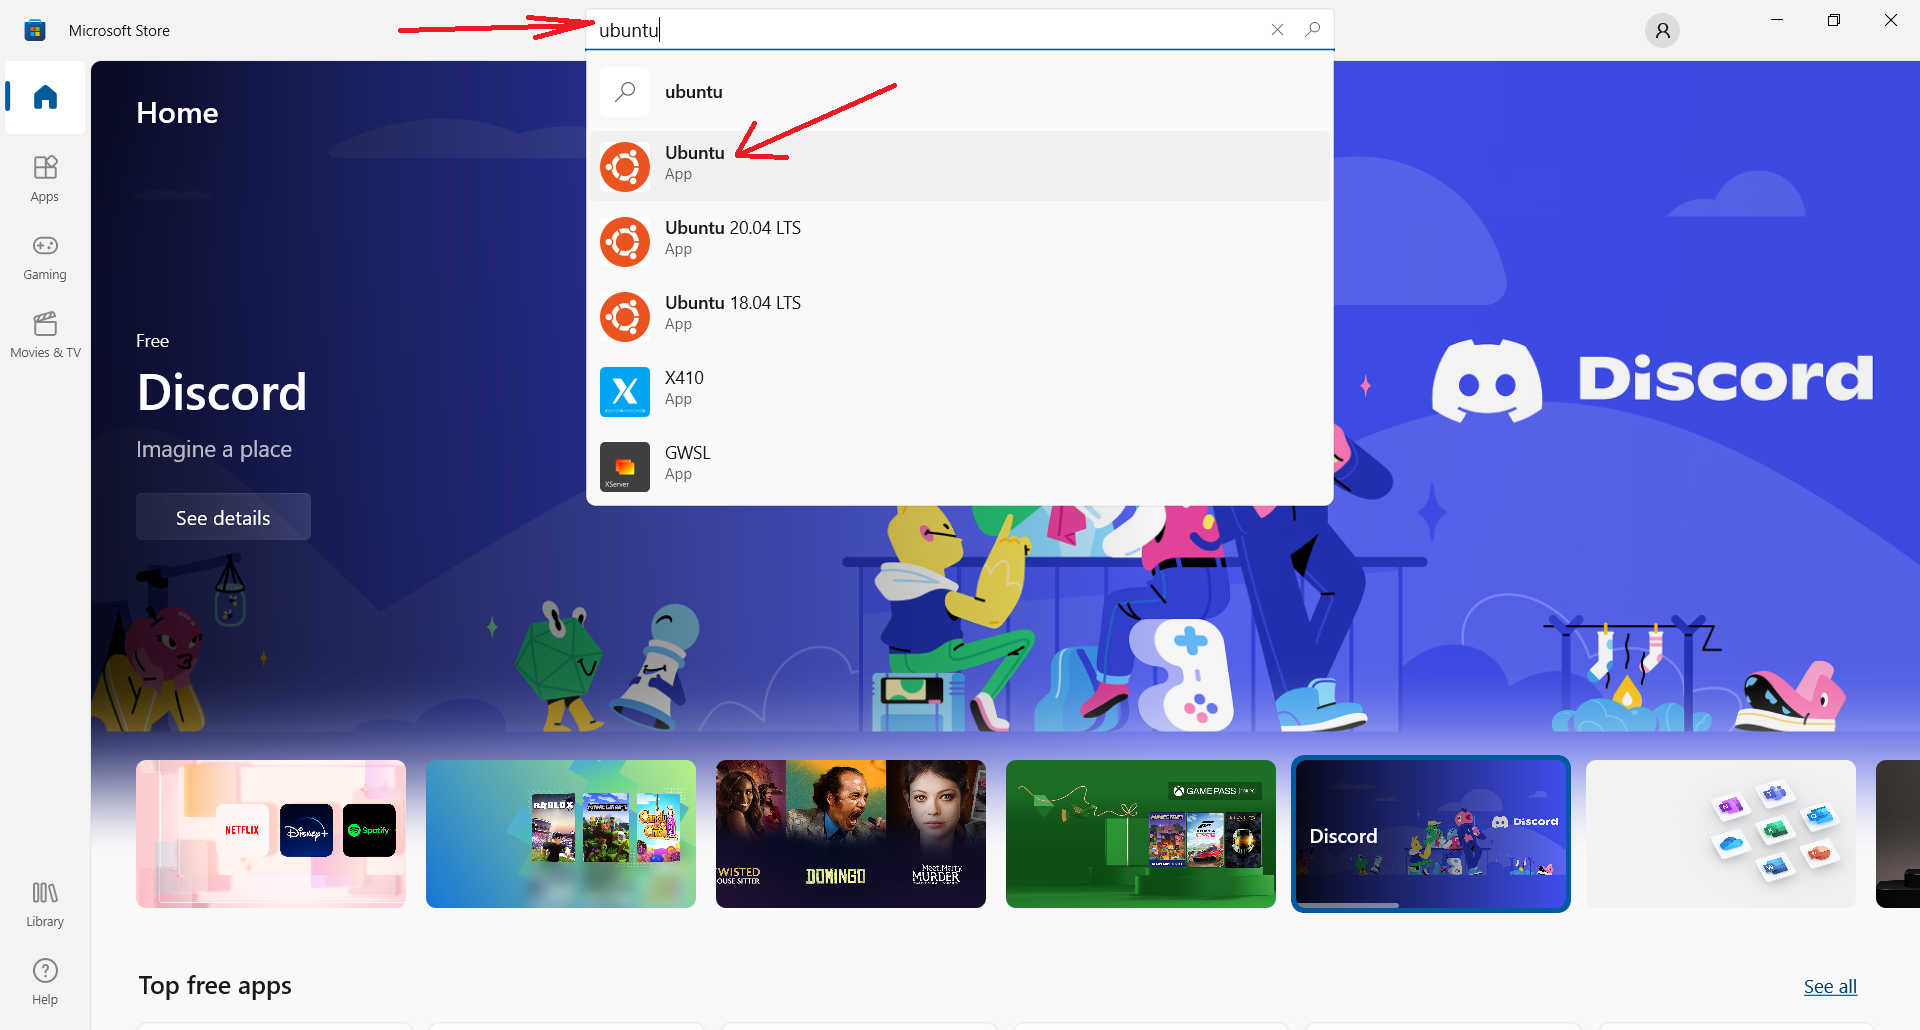
\includegraphics[width=\linewidth]
            {_assets/gpi_pz_docker_17.png}
        \caption{Открываем поиск, вводим <<Ubuntu>> и выбираем подходящий вариант}
        \label{fig:gpi_pz_docker_17}
    \end{minipage}
    \begin{minipage}{0.47\textwidth}
        \centering
        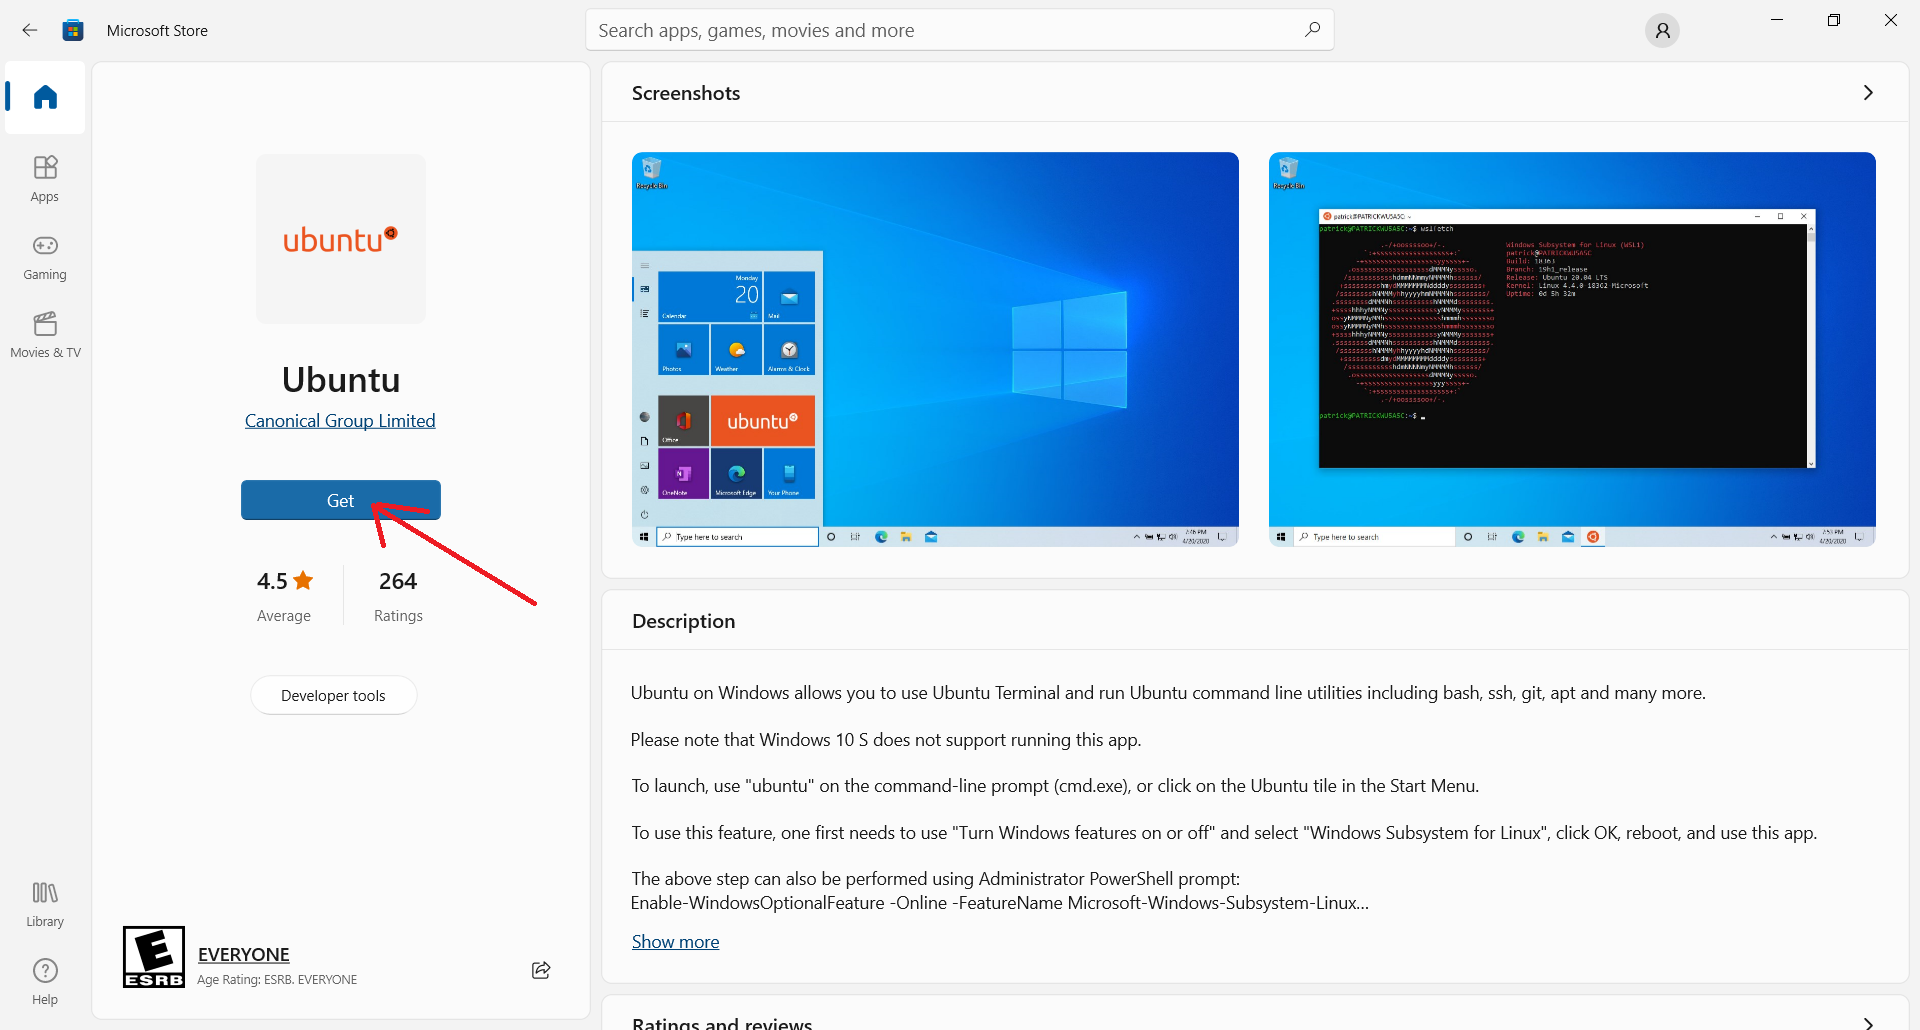
\includegraphics[width=\linewidth]
            {_assets/gpi_pz_docker_18.png}
        \caption{Устанавливаем приложение, нажав на кнопку <<Get>>}
        \label{fig:gpi_pz_docker_18}
    \end{minipage}
\end{figure}

\begin{figure}[!p]
    \centering
    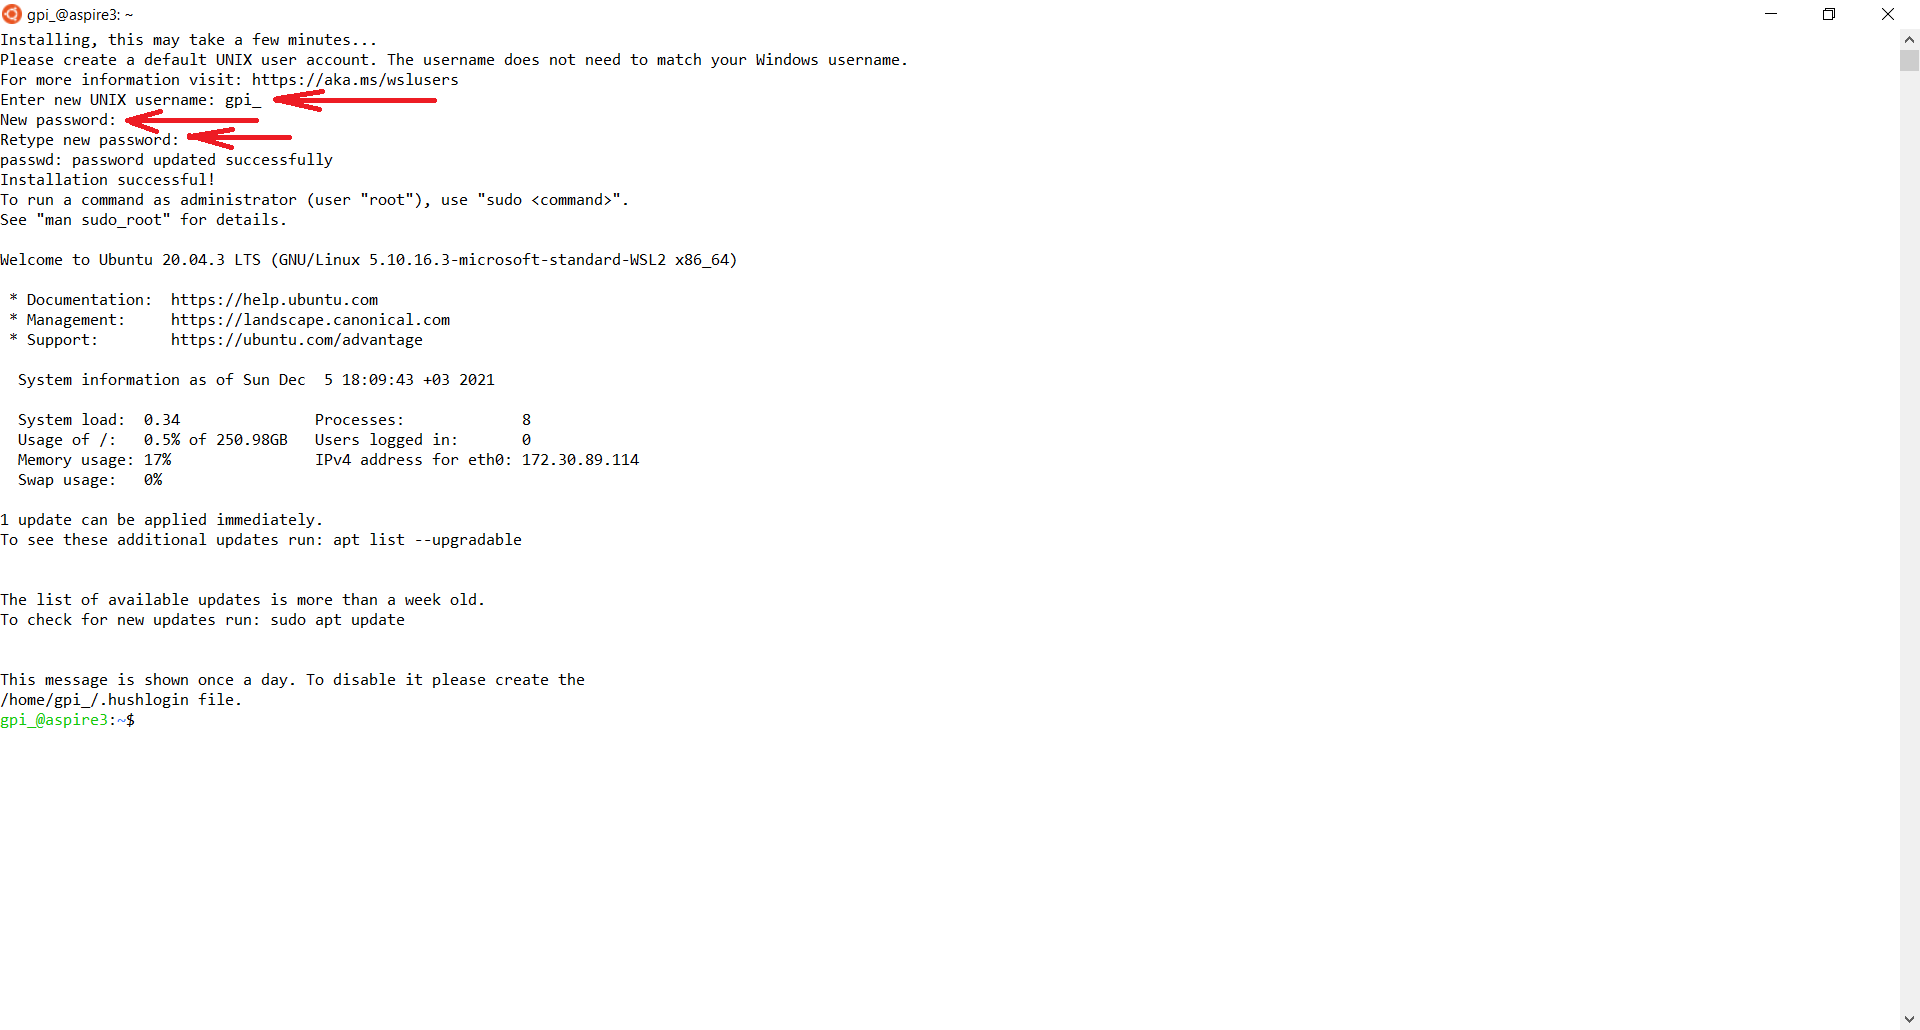
\includegraphics[width=12cm]
        {_assets/gpi_pz_docker_19.png}
    \caption{При первом запуске устанавливаем имя пользователя и пароль для дистрибутива}
    \label{fig:gpi_pz_docker_19}
\end{figure}

\begin{figure}[!p]
    \centering
    \begin{minipage}{0.47\textwidth}
        \centering
        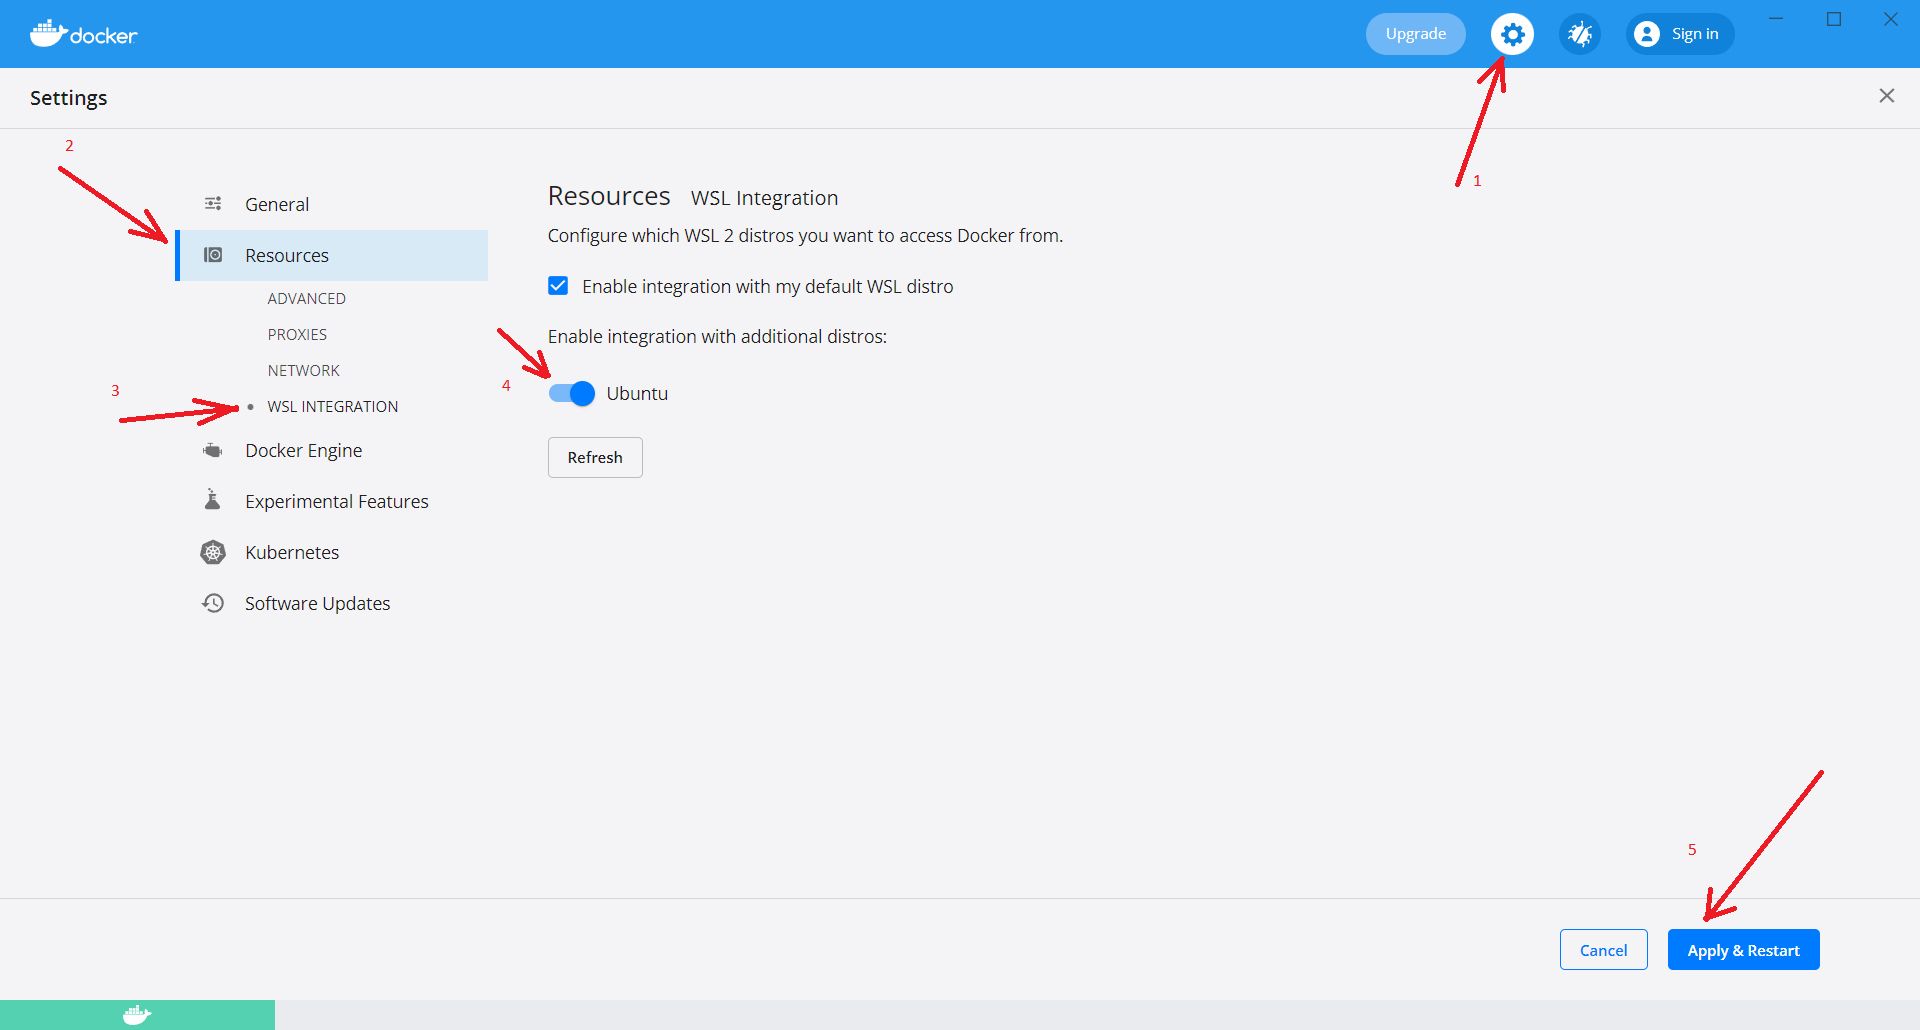
\includegraphics[width=\linewidth]
            {_assets/gpi_pz_docker_20.png}
        \caption{Включаем в приложении работу в дистрибутиве <<Ubuntu>>}
        \label{fig:gpi_pz_docker_20}
    \end{minipage}
    \begin{minipage}{0.47\textwidth}
        \centering
        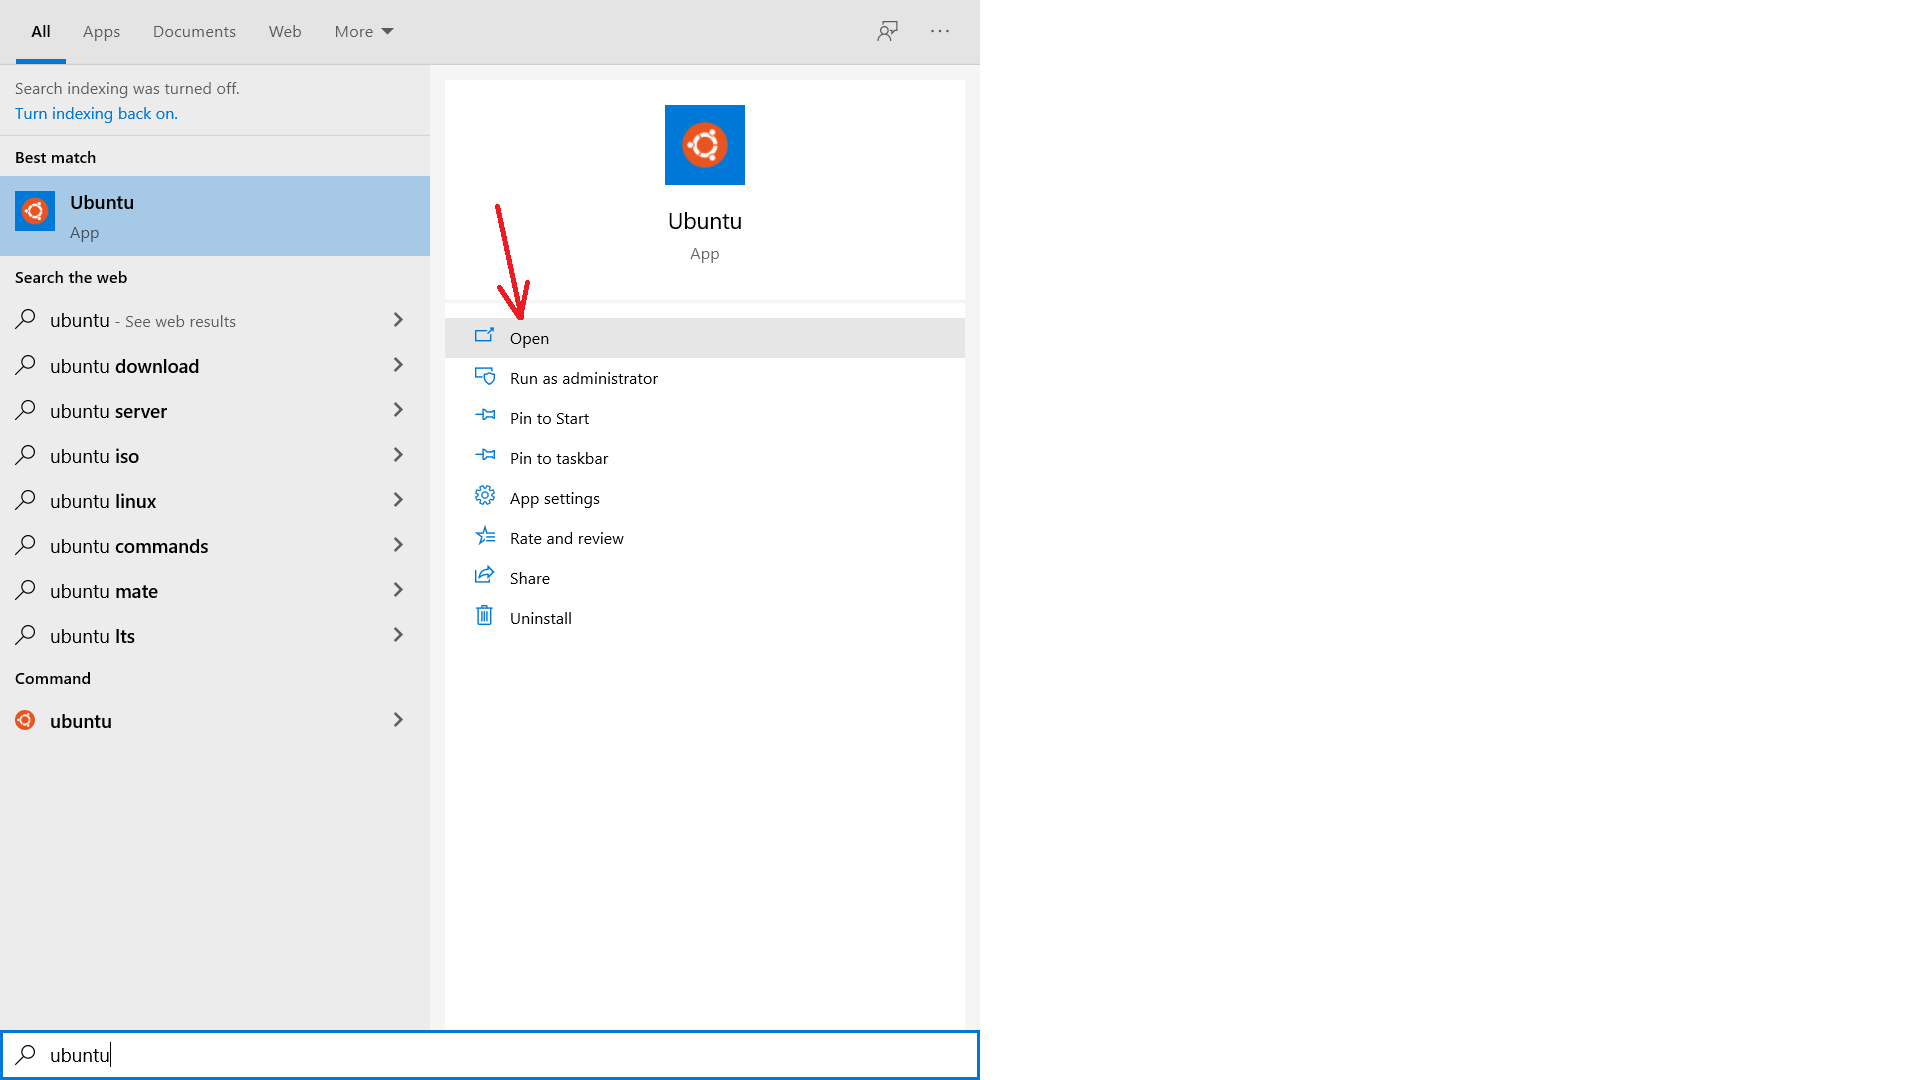
\includegraphics[width=\linewidth]
            {_assets/gpi_pz_docker_21.png}
        \caption{Зажимаем <<Win>> + <<Q>> и в поиске вводим <<Ubuntu>>}
        \label{fig:gpi_pz_docker_21}
    \end{minipage}
\end{figure}

\begin{figure}[!p]
    \centering
    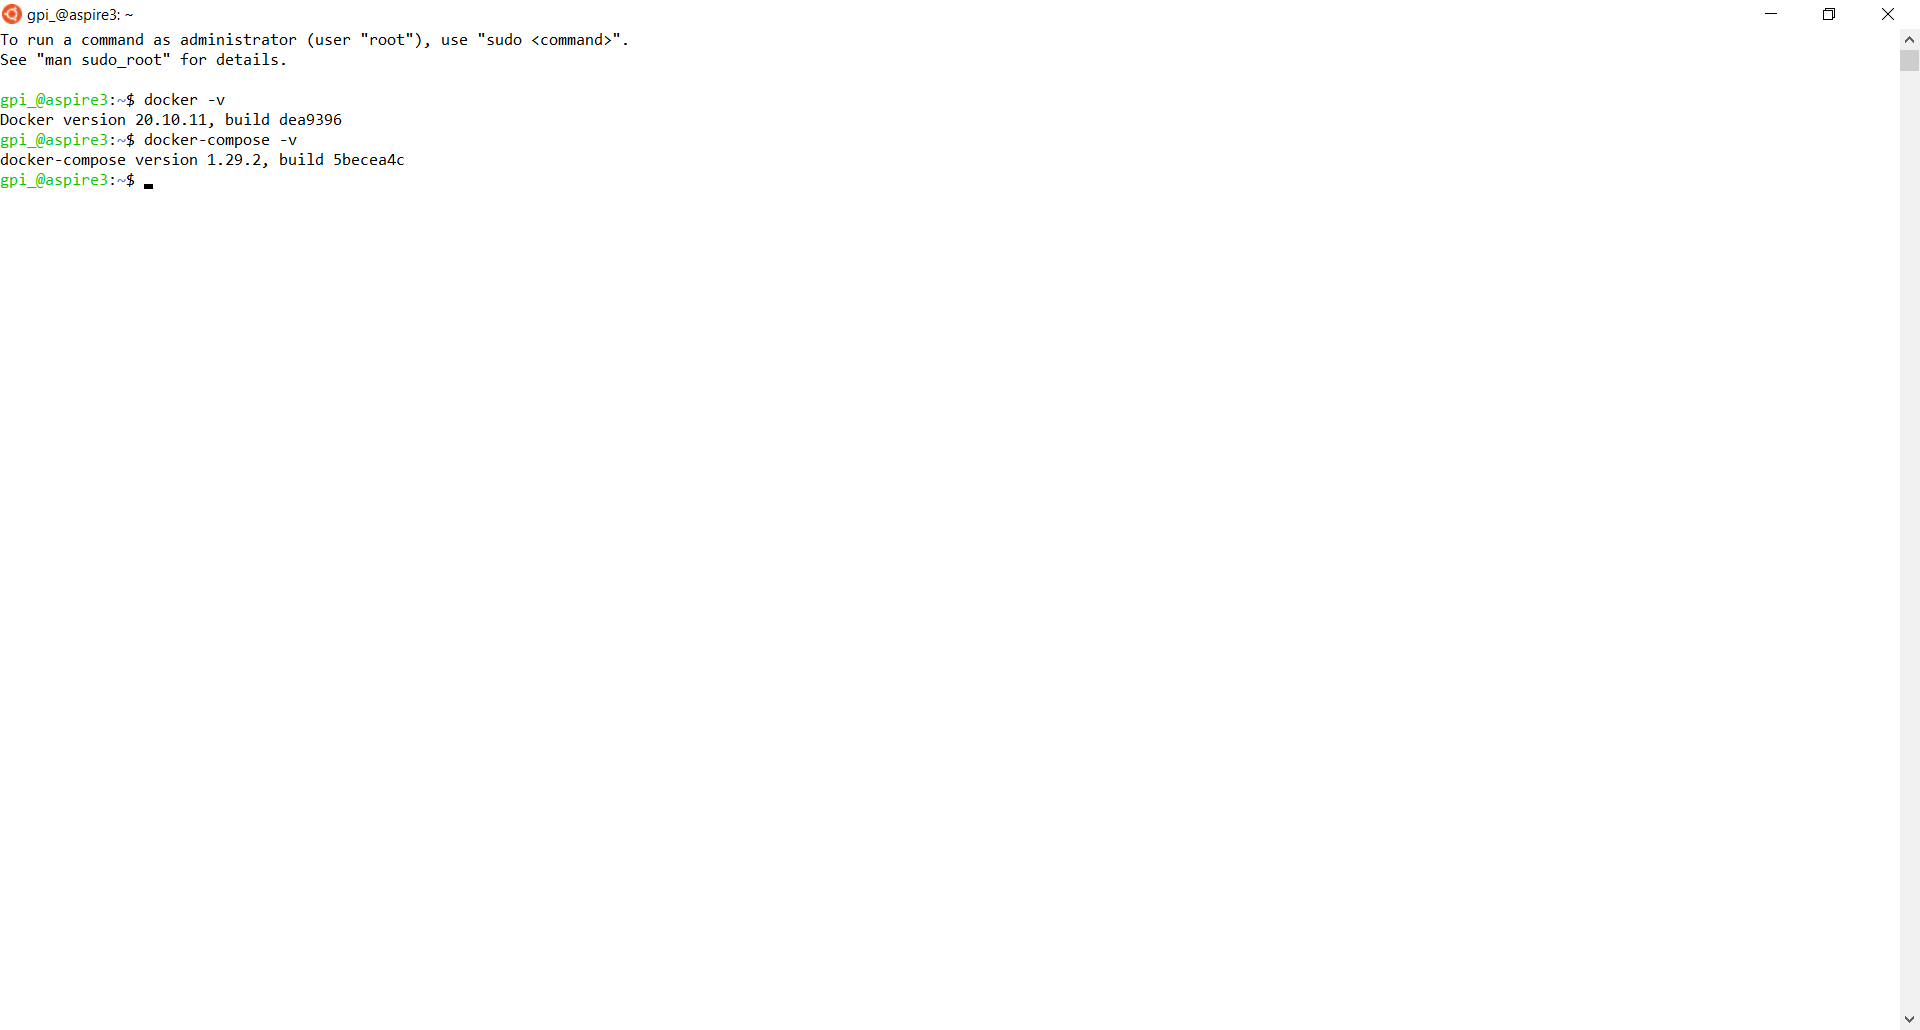
\includegraphics[width=12cm]
        {_assets/gpi_pz_docker_22.png}
    \caption{Убеждаемся в установке Docker, проверив версию Docker и docker-compose}
    \label{fig:gpi_pz_docker_22}
\end{figure}

\subsubsection*{Установка docker на Linux}

\begin{itemize}
    \item[1.] <<sudo apt update>> - обновляем базу пакетов.
    \item[2.] <<sudo apt install docker.io>> - устанавливаем docker.
    \item[3.] <<sudo apt install docker-compose>> - устанавливаем docker-compose.
\end{itemize}

\newpage

% = = = = = = = = = = = = = = = =

\subsection{Скрипты для запуска (Makefile)}

\subsubsection*{Установка make на Windows 10}

Для установки make в Windows 10 нужен пакетный менеджер <<choco>>. Установим его.

\begin{itemize}
    \item[1.] Заходим на официальный сайт choco:
    \url{https://chocolatey.org/} \\
    Жмём кнопку <<Get Started>>. \\
    Скриншот на \textbf{рис.~\ref{fig:gpi_pz_choco_1} (стр. \pageref{fig:gpi_pz_choco_1})}.

    \item[2.] Появляемся на странице с инструкцией, на которой есть скрипт Power Shell.
    Копируем это скрипт. \\
    Скриншот на \textbf{рис.~\ref{fig:gpi_pz_choco_2} (стр. \pageref{fig:gpi_pz_choco_2})}.

    \item[3.] Откроем Power Shell через поиск.
    Для открытия поиска жмём <<Win>> + <<R>>.
    В поиске вводим <<powershell>>.
    Открывать нужно от имени администратора.
    Жмём кнопку <<Run as Administrator>>. \\
    Скриншот на \textbf{рис.~\ref{fig:gpi_pz_choco_3} (стр. \pageref{fig:gpi_pz_choco_3})}.

    \item[4.] В Power Shell вставляем скопированный скрипт. \\
    Скриншот на \textbf{рис.~\ref{fig:gpi_pz_choco_4} (стр. \pageref{fig:gpi_pz_choco_4})}.

    \item[5.] Откроем Power Shell через поиск.
    Для открытия поиска жмём <<Win>> + <<R>>.
    В поиске вводим <<powershell>>.
    Открывать нужно от имени администратора.
    Жмём кнопку <<Run as Administrator>>. \\
    Скриншот на \textbf{рис.~\ref{fig:gpi_pz_choco_5} (стр. \pageref{fig:gpi_pz_choco_5})}.

    \item[6.] В Power Shell прописываем <<choco install make>> - и жмём <<Enter>>.
    После установки проверяем введя <<make -v>>. \\
    Скриншот на \textbf{рис.~\ref{fig:gpi_pz_choco_6} (стр. \pageref{fig:gpi_pz_choco_6})}.

\end{itemize}

\begin{figure}[!p]
    \centering
    \begin{minipage}{0.47\textwidth}
        \centering
        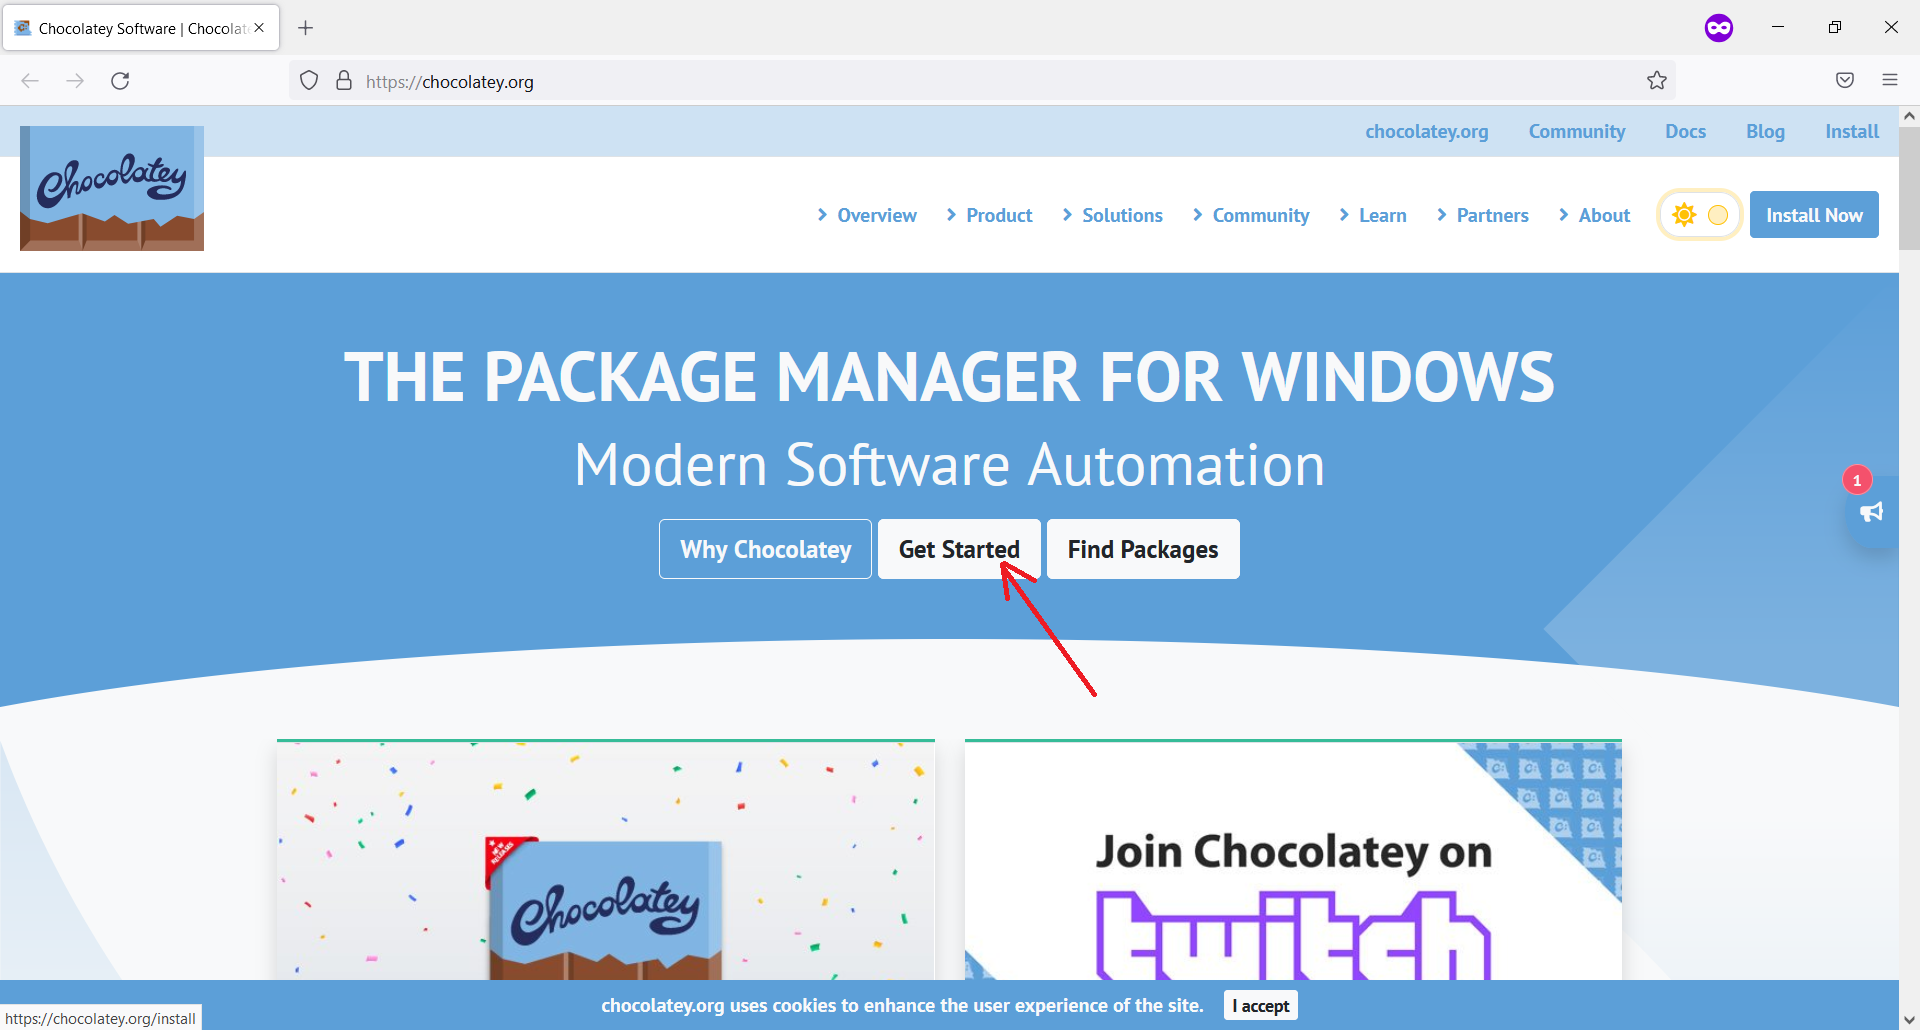
\includegraphics[width=\linewidth]
            {_assets/gpi_pz_choco_1.png}
        \caption{На сайте choco жмём <<Get Started>>}
        \label{fig:gpi_pz_choco_1}
    \end{minipage}
    \begin{minipage}{0.47\textwidth}
        \centering
        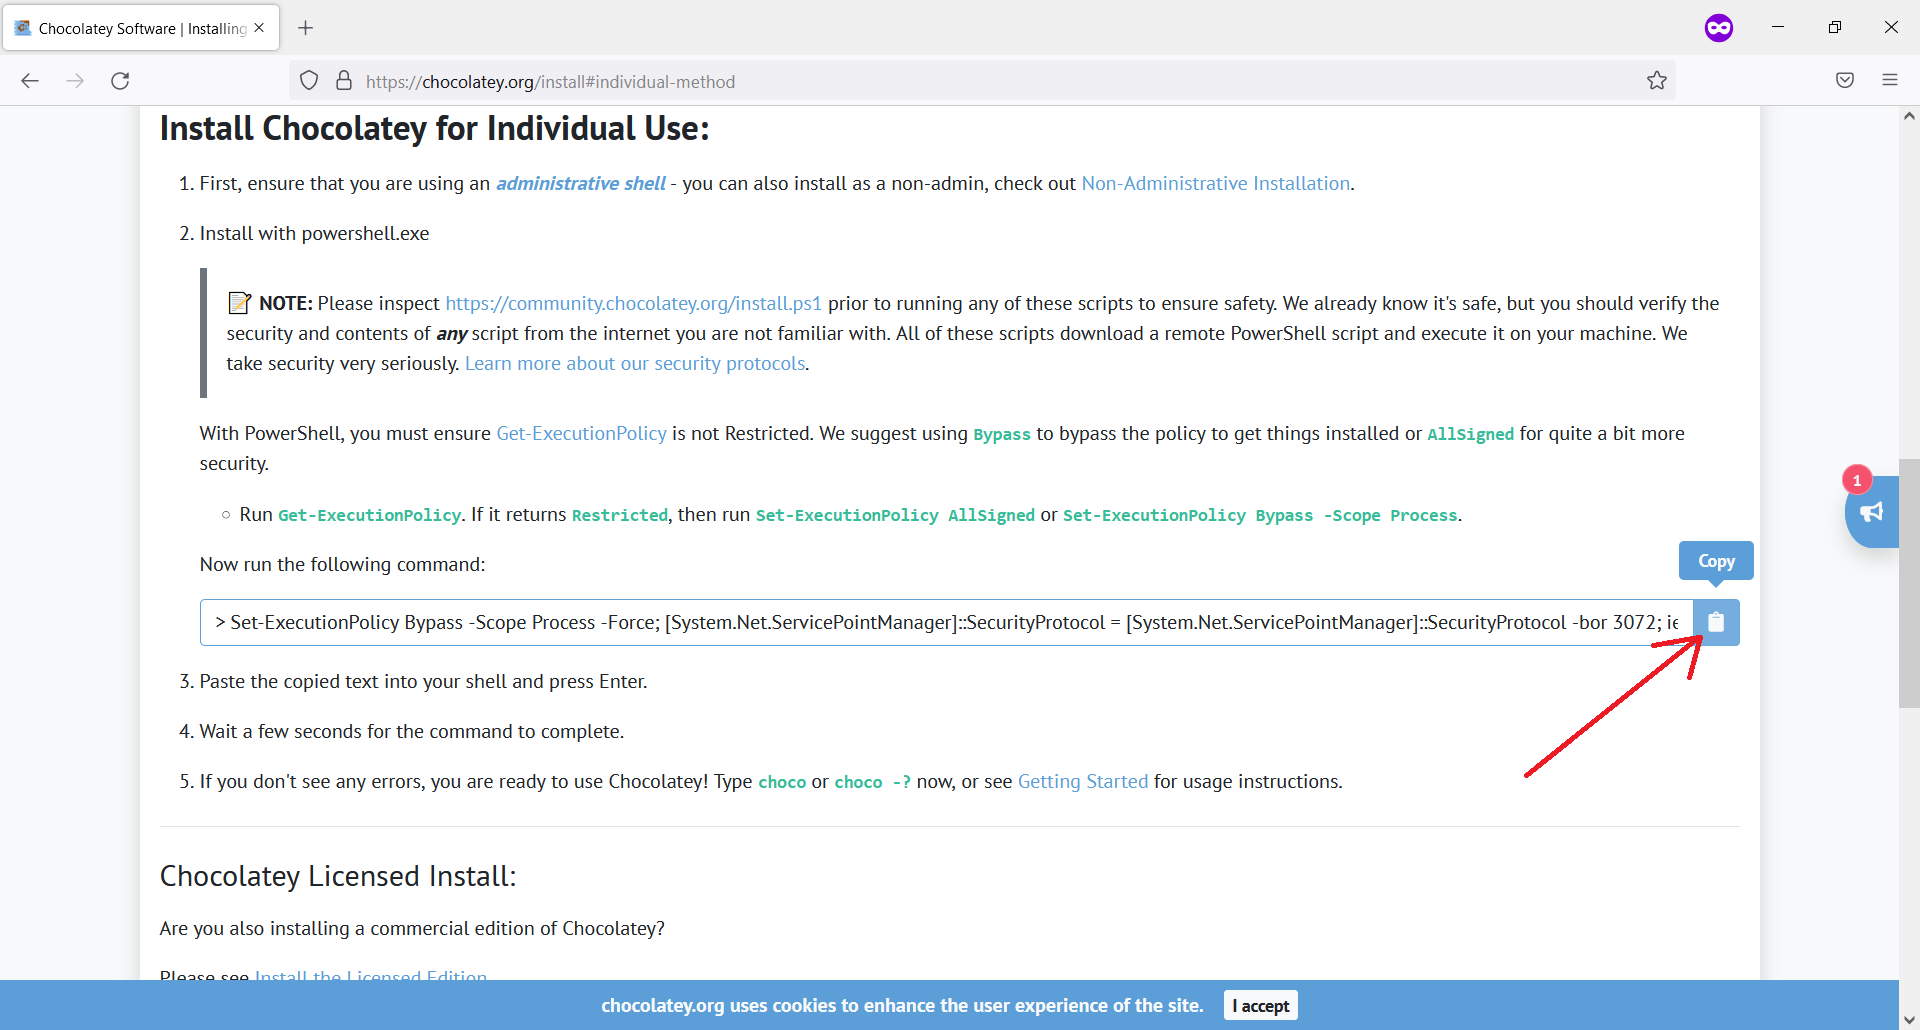
\includegraphics[width=\linewidth]
            {_assets/gpi_pz_choco_2.png}
        \caption{На сайте с инструкцией choco копируем скрипт}
        \label{fig:gpi_pz_choco_2}
    \end{minipage}
\end{figure}

\begin{figure}[!p]
    \centering
    \begin{minipage}{0.47\textwidth}
        \centering
        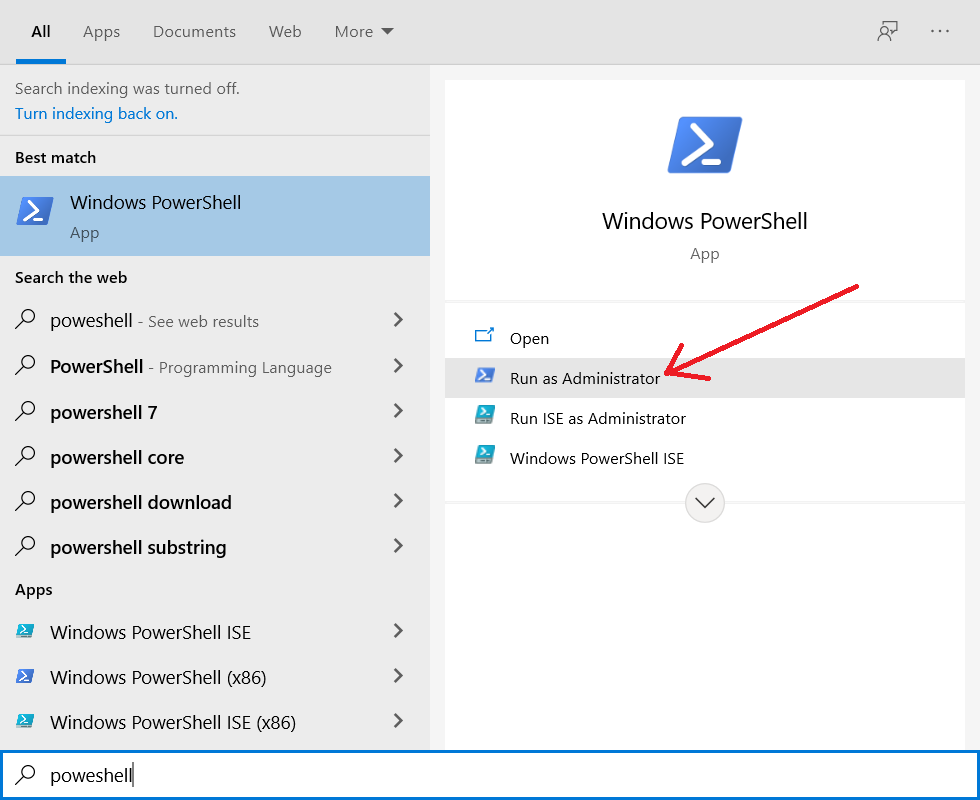
\includegraphics[width=\linewidth]
            {_assets/gpi_pz_choco_3.png}
        \caption{Жмём <<Win>> + <<Q>>. Вводим в поиск <<powershell>>. Открываем от имени администратора}
        \label{fig:gpi_pz_choco_3}
    \end{minipage}
    \begin{minipage}{0.47\textwidth}
        \centering
        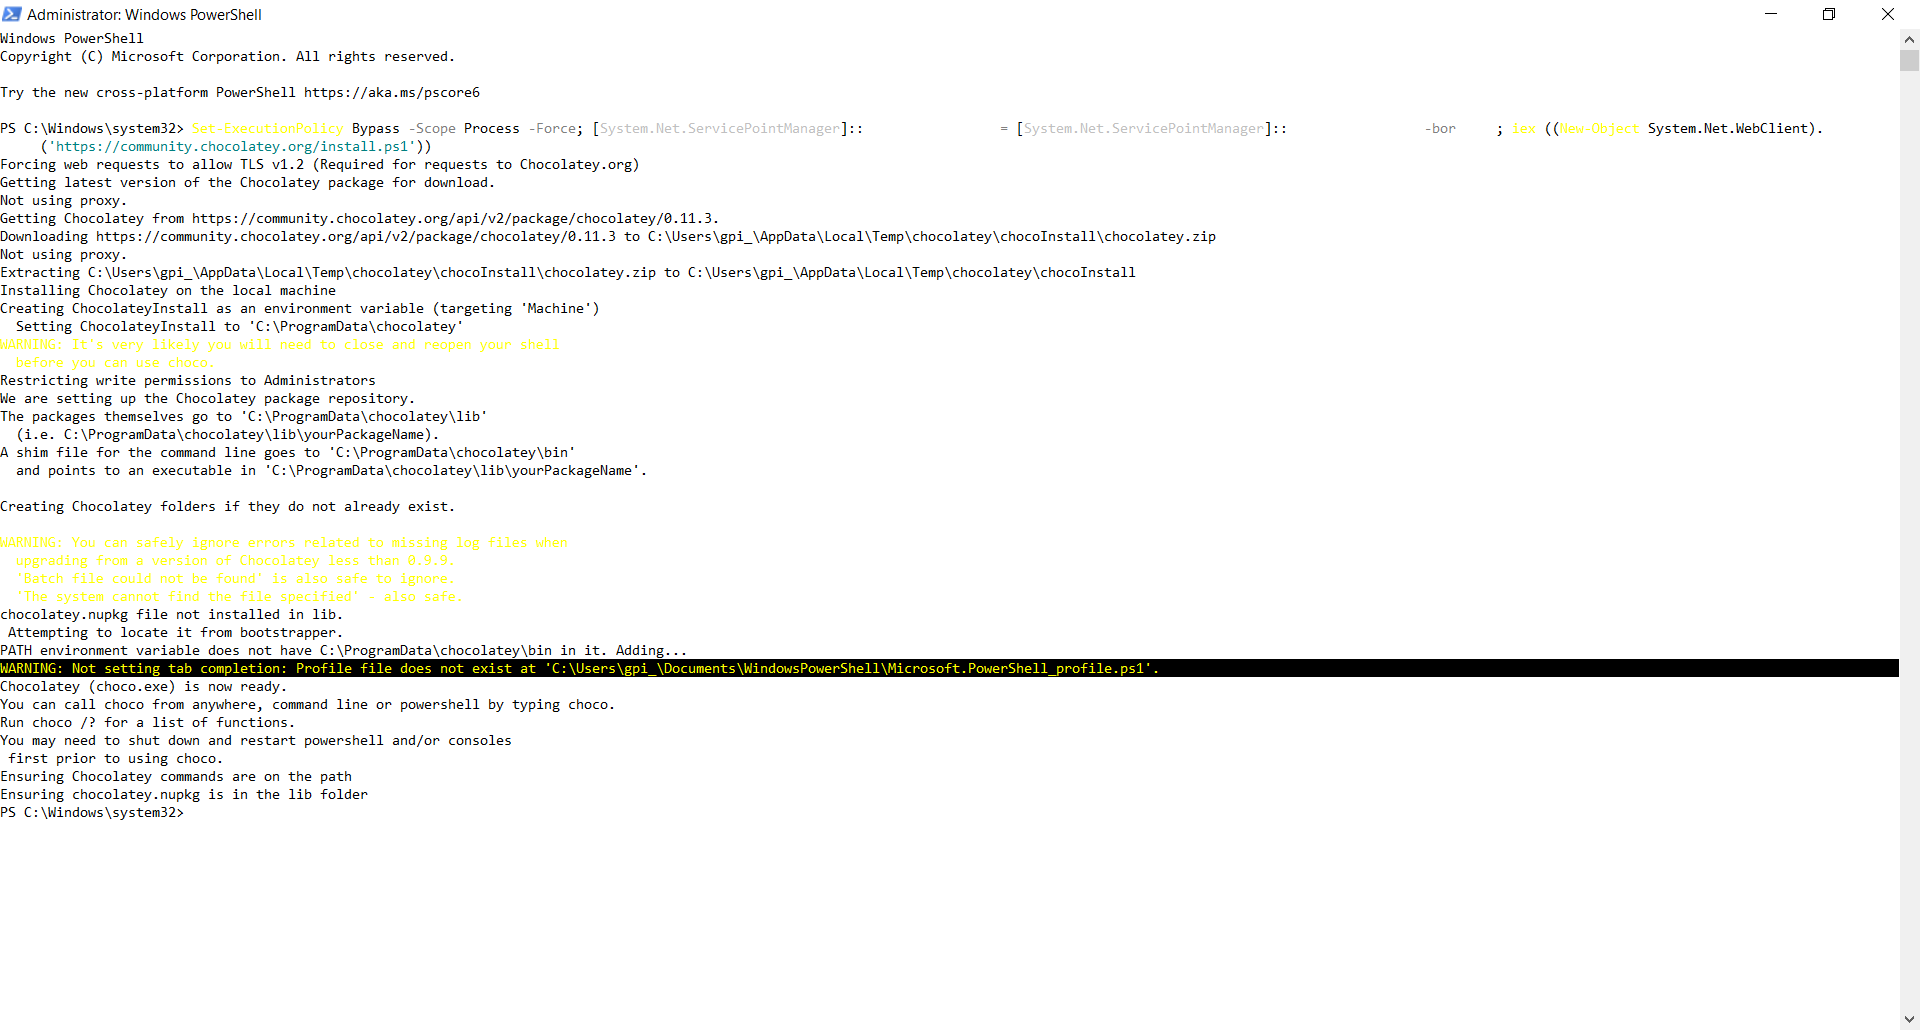
\includegraphics[width=\linewidth]
            {_assets/gpi_pz_choco_4.png}
        \caption{В PowerShell вставляем скопированный скрипт. Жмём <<Enter>>. Жмём установки choco}
        \label{fig:gpi_pz_choco_4}
    \end{minipage}
\end{figure}

\begin{figure}[!p]
    \centering
    \begin{minipage}{0.47\textwidth}
        \centering
        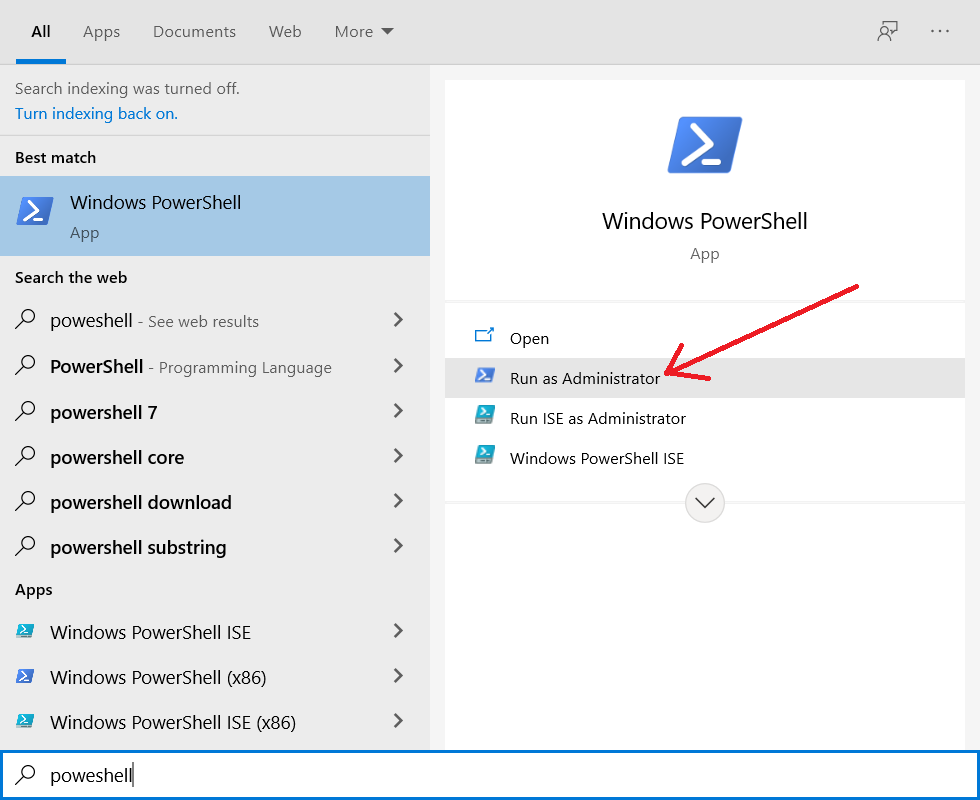
\includegraphics[width=\linewidth]
            {_assets/gpi_pz_choco_5.png}
        \caption{Жмём <<Win>> + <<Q>>. Вводим в поиск <<powershell>>. Открываем от имени администратора}
        \label{fig:gpi_pz_choco_5}
    \end{minipage}
    \begin{minipage}{0.47\textwidth}
        \centering
        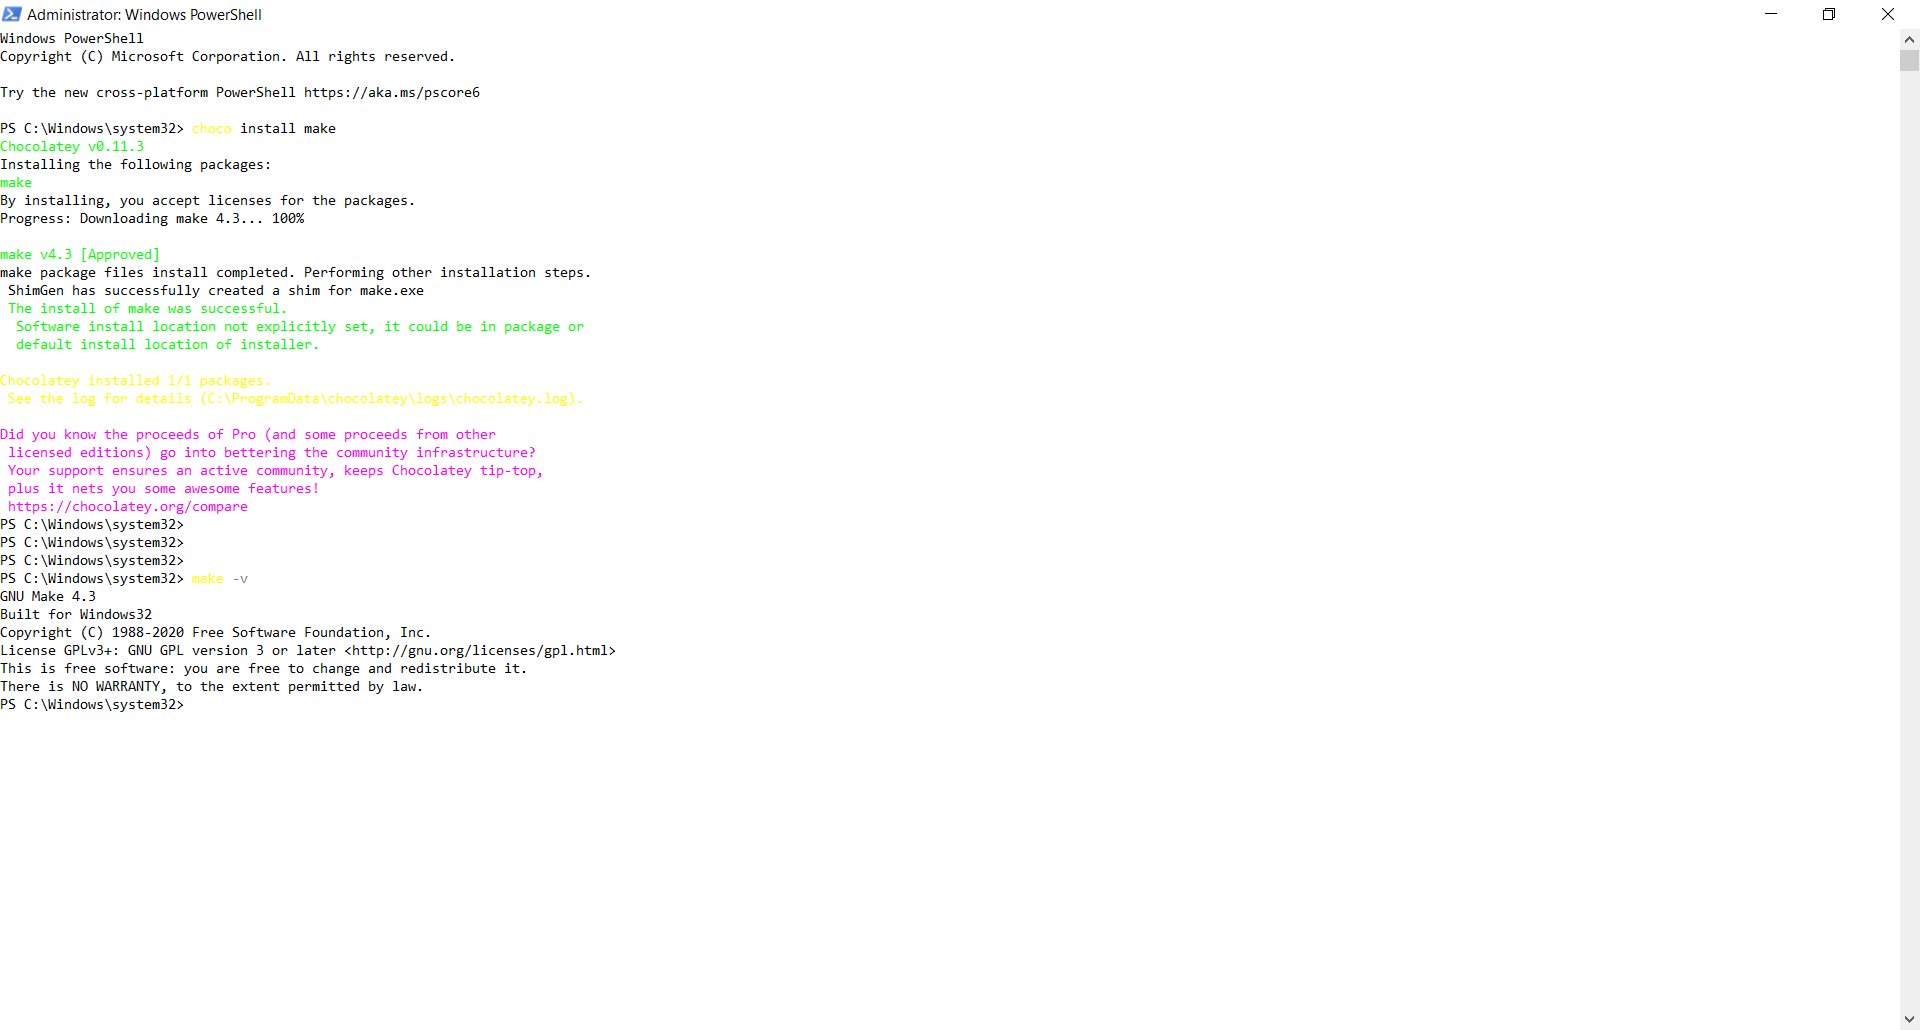
\includegraphics[width=\linewidth]
            {_assets/gpi_pz_choco_6.png}
        \caption{В PowerShell вставляем скрипт <<choho make install>>. Жмём <<Enter>>. Жмём установки make.
        Проверяем установку введя <<make -v>>}
        \label{fig:gpi_pz_choco_6}
    \end{minipage}
\end{figure}

% = = = = = = = = = = = = = = = =

\subsubsection*{Установка make на Linux}

\begin{itemize}
    \item[1.] <<sudo apt update>> - обновляем базу пакетов.
    \item[2.] <<sudo apt install make>> - устанавливаем make.
\end{itemize}

\newpage

% = = = = = = = = = = = = = = = =

\subsubsection*{Скрипты для запуска проектов}

Для того чтобы запускать каждый проект нужно входить в каждую папку проекта и запускать скрипт.
Заходить в каждую папку и прописывать опеределеную команду занимала много времени.
Было принято решение записать все команды в Makefile.

\begin{table}[!h]
    \centering
    \caption{Makefile команды}
    \begin{tabular}{|p{4cm}|p{12cm}|}

                                                                                   \hline
\multicolumn{1}{|c|}{\textbf{Команда}} & \multicolumn{1}{c|}{\textbf{Описание}} \\ \hline
make gpi\_wi    & cmd: установки пакетов для проектов npm                       \\ \hline 
make gpi\_wc    & cmd: копирования env файлов                                   \\ \hline  
make gpi\_wb    & cmd: запуск Express сервера                                   \\ \hline
make gpi\_wfa   & cmd: запуск React приложения с админа панелью                 \\ \hline
make gpi\_wfs   & cmd: запуск React приложения с магазином                      \\ \hline
make gpi\_wm    & cmd: запуск MySQL через Docker                                \\ \hline
make gpi\_wp    & cmd: компиляция PDF файлов через LaTeX                        \\ \hline

    \end{tabular}
\end{table}

\subsection{Описание проектов}

\begin{table}[!h]
    \centering
    \caption{Разрабатываемые проекты}
    \begin{tabular}{|p{4cm}|p{4cm}|p{8cm}|}

                                                                                           \hline
\multicolumn{1}{|c|}{\textbf{Папка проекта}}& \multicolumn{2}{c|}{\textbf{Описание}}    \\ \hline
gpi\_b  & Backend API           & Node JS Express cервер возвращает JSON                \\ \hline 
gpi\_d  & JSON object array     & Пример файла для загрузки в БД                        \\ \hline  
gpi\_fa & Frontend adminpanel   & React JS cайт админка                                 \\ \hline  
gpi\_fs & Frontend webstore     & React JS cайт магазин                                 \\ \hline
gpi\_m  & MySQL                 & Docker LAMP база данных                               \\ \hline
gpi\_p  & PDF documents         & LaTeX для cоздания ЕСКД отчётов                       \\ \hline

    \end{tabular}
\end{table}

\newpage
